%%
%% This is file `mathexample.tex',
%% generated with the docstrip utility.
%%
%% The original source files were:
%%
%% texpower-doc.dtx  (with options: `mathexample,mathexample-src,end')
%% 
%% --------------------------------------------------------------
%% TeXPower bundle - dynamic online presentations with LaTeX
%% Copyright (C) 1999-2004 Stephan Lehmke
%% Copyright (C) 2003-2005 Hans Fredrik Nordhaug
%% 
%% This program is free software; you can redistribute it and/or
%% modify it under the terms of the GNU General Public License
%% as published by the Free Software Foundation; either version 2
%% of the License, or (at your option) any later version.
%% 
%% This program is distributed in the hope that it will be useful,
%% but WITHOUT ANY WARRANTY; without even the implied warranty of
%% MERCHANTABILITY or FITNESS FOR A PARTICULAR PURPOSE.  See the
%% GNU General Public License for more details.
%% --------------------------------------------------------------
%% 
%% The list of all files belonging to the TeXPower bundle is
%% given in the file `00readme.txt'.
%% 
\ProvidesFile{talk.tex}%
      [2005/04/07 TeXPower example file]
%-----------------------------------------------------------------------------------------------------------------
%
% Math example for the package texpower.sty.
%
%-----------------------------------------------------------------------------------------------------------------
% Enable all color emphasis and highlighting options. Use white background and slifonts.

\PassOptionsToPackage{coloremph,colormath,colorhighlight,lightbackground}{texpower}

% Input the generic preamble.

%\input{__TPpreamble}
\documentclass[12pt,letterpaper,landscape,KOMA,smallheadings,calcdimensions,display]{powersem}

\usepackage{tpslifonts}
%-----------------------------------------------------------------------------------------------------------------
% We load hyperref and fixseminar which fixes some problems with seminar.
%
\usepackage[ps2pdf,plainpages=false,bookmarksopen,colorlinks,pdfpagemode=FullScreen]{hyperref}
\usepackage{seminar}
\usepackage{fixseminar}

%-----------------------------------------------------------------------------------------------------------------
% Finally, the texpower package is loaded.
%
\usepackage{texpower}
\usepackage{soul}


% We write some aligned equations.

\usepackage{amsmath}
\usepackage{amssymb}
\usepackage{relsize}
\usepackage[pdftex]{graphicx}
% Make nested braces grow.
\delimitershortfall-1sp

%-----------------------------------------------------------------------------------------------------------------
% Finally, everything is set up. Here we go...
%

\newcommand{\beq}{\begin{equation}}
\newcommand{\eeq}{\end{equation}}


\def\ie{{\it i.e.}}
\def\eg{{\it e.g.}}
\newcommand{\p}{\partial}
\newcommand{\mc}[1]{\mathcal{#1}}
\newcommand{\md}{\mathcal{D}}
\newcommand{\wt}{\widetilde}
\newcommand{\ov}{\overline}
\newcommand{\suc}{{\rm SU}_{\rm C}(3)}
\newcommand{\sul}{{\rm SU}_{\rm L}(2)}
\newcommand{\ue}{{\rm U}(1)}
\newcommand{\GeV}{{\rm GeV}}
\newcommand{\eV}{{\rm eV}}
\newcommand{\ha}{\frac{1}{2}}
%\newcommand{\su3}{{\rm SU}_{\rm C}(3)}
%%%%%%%%%%%%%%%%%%%%%%%%%%%%%%%%%%%%%%%
%  Slash character...
\def\slashed#1{\setbox0=\hbox{$#1$}             % set a box for #1
   \dimen0=\wd0                                 % and get its size
   \setbox1=\hbox{/} \dimen1=\wd1               % get size of /
   \ifdim\dimen0>\dimen1                        % #1 is bigger
      \rlap{\hbox to \dimen0{\hfil/\hfil}}      % so center / in box
      #1                                        % and print #1
   \else                                        % / is bigger
      \rlap{\hbox to \dimen1{\hfil$#1$\hfil}}   % so center #1
      /                                         % and print /
   \fi}                                        %
%%EXAMPLE:  $\slashed{E}$ or $\slashed{E}_{t}$

\newcommand{\LUV}{\Lambda_{\rm UV}}


\newcommand{\lgr}{\left\lgroup}
\newcommand{\rgr}{\right\rgroup}




%-----------------------------------------------------------------------------------------------------------------
% Set slide margins rather small for maximum use of space. 
%
\renewcommand{\slidetopmargin}{15mm}
\renewcommand{\slidebottommargin}{5mm}

\renewcommand{\slideleftmargin}{5mm}
\renewcommand{\sliderightmargin}{5mm}
\renewcommand\section{\@startsection{section}{1}{\z@}%
  {-1.5ex\@plus -1ex \@minus -.5ex}%
  {.5ex \@plus .2ex}%
  {\raggedsection\normalfont\size@section\sectfont}}

\renewcommand\subsection{\@startsection{subsection}{2}{\z@}%
  {-1.25ex\@plus -1ex \@minus -.2ex}%
  {.5ex \@plus .2ex}%
  {\raggedsection\normalfont\size@subsection\sectfont}}

\renewcommand\subsubsection{\@startsection{subsubsection}{3}{\z@}%
  {-1.25ex\@plus -1ex \@minus -.2ex}%
  {.5ex \@plus .2ex}%
  {\raggedsection\normalfont\size@subsubsection\sectfont}}

\renewcommand\paragraph{\@startsection{paragraph}{4}{\z@}%
  {1.25ex \@plus1ex \@minus.2ex}%
  {-1em}%
  {\raggedsection\normalfont\size@paragraph\sectfont}}

\def\slideitemsep{.5ex plus .3ex minus .2ex}


\slideframe{none}


\newcommand{\sunu}{SU(N) \times U(1)}
\newcommand{\aU}{a^{\rm U(1)}}
\newcommand{\aN}{a^{\rm SU(N)}}
\newcommand{\lU}{\lambda^{\rm U(1)}}
\newcommand{\lN}{\lambda^{\rm SU(N)}}
\newcommand{\Tr}{{\rm Tr\,}}
\newcommand{\bxir}{\ov{\xi}{}_R}
\newcommand{\bxil}{\ov{\xi}{}_L}
\newcommand{\xir}{\xi_R}
\newcommand{\xil}{\xi_L}
\newcommand{\bzl}{\ov{\zeta}{}_L}
\newcommand{\bzr}{\ov{\zeta}{}_R}
\newcommand{\zr}{\zeta_R}
\newcommand{\zl}{\zeta_L}
\newcommand{\nbar}{\ov{n}}
\newcommand{\nfour}{${\cal N}=4\;$}
\newcommand{\ntwo}{${\mathcal N}=2\;$}
\newcommand{\none}{${\mathcal N}=1\,$}
\newcommand{\ntt}{${\mathcal N}=(2,2)\,$}
\newcommand{\nzt}{${\mathcal N}=(0,2)\,$}
\newcommand{\cpn}{CP$(N-1)\,$}
\newcommand{\ca}{{\mathcal A}}
\newcommand{\cell}{{\mathcal L}}
\newcommand{\cw}{{\mathcal W}}
\newcommand{\cs}{{\mathcal S}}
\newcommand{\vp}{\varphi}
\newcommand{\pt}{\partial}
\newcommand{\ve}{\varepsilon}
\newcommand{\gs}{g^{2}}
\newcommand{\zn}{$Z_N$}
\newcommand{\cd}{${\mathcal D}$}
\newcommand{\cde}{{\mathcal D}}
\newcommand{\cf}{${\mathcal F}$}
\newcommand{\cfe}{{\mathcal F}}

\newcommand{\mbps}{m_{\text{\tiny BPS}}}
\newcommand{\W}{\mathcal{W}}
\newcommand{\hsigma}{{\hat{\sigma}}}


\usepackage[T1]{fontenc}
\renewcommand*\ttdefault{lmvtt}
\renewcommand*\familydefault{\ttdefault} %% Only if the base font of the document is to be typewriter style

\newcommand{\sectionfont}{
\usefont{OT1}{lmvtt}{b}{n}\fontsize{45pt}{30pt}\selectfont
\bfseries}
\backgroundstyle{vgradient}


\begin{document}

%%%%%%%%%%%%%%%%%%%%%%%%%%%%%%%%%%%%%%%%%%%%%%%%%%%%%%%%%%%%%%%%%%%%%%%%%%%%%%%%%%%%%
%%%%%%%%%%%%%%%%%%%%%%%%%%%%%%%%%%%%%%%%%%%%%%%%%%%%%%%%%%%%%%%%%%%%%%%%%%%%%%%%%%%%%
\begin{slide}

\begin{center}

\vspace*{1.7cm}
{\Large Curves of Marginal Stability in\\[2mm]
    Supersymmetric CP($N-1$) theory with\\[3.5mm]
	$ \mc{Z}_N $ twisted masses}

\vspace{1.4cm}

{Pavel A. Bolokhov\\
\small
~~~~FTPI, University of Minnesota}

{\small In collaboration with M.Shifman and A.Yung}

\end{center}

\end{slide}


%%%%%%%%%%%%%%%%%%%%%%%%%%%%%%%%%%%%%%%%%%%%%%%%%%%%%%%%%%%%%%%%%%%%%%%%%%%%%%%%%%%%%
%%%%%%%%%%%%%%%%%%%%%%%%%%%%%%%%%%%%%%%%%%%%%%%%%%%%%%%%%%%%%%%%%%%%%%%%%%%%%%%%%%%%%
\begin{slide}

\begin{center}

\vspace*{0.58cm}
{\Large    The BPS Spectrum and\\[2mm]
	Curves of Marginal Stability in\\[2mm]
    Supersymmetric CP($N-1$) theory with\\[3.5mm]
	$ \mc{Z}_N $ twisted masses}

\vspace{1.4cm}

{Pavel A. Bolokhov\\
\small
~~~~FTPI, University of Minnesota}

{\small In collaboration with M.Shifman and A.Yung}

\end{center}

\end{slide}



%%%%%%%%%%%%%%%%%%%%%%%%%%%%%%%%%%%%%%%%%%%%%%%%%%%%%%%%%%%%%%%%%%%%%%%%%%%%%%%%%%%%%
%%%%%%%%%%%%%%%%%%%%%%%%%%%%%%%%%%%%%%%%%%%%%%%%%%%%%%%%%%%%%%%%%%%%%%%%%%%%%%%%%%%%%
\begin{slide}

\vspace*{3.0cm} 
\begin{center}
\usefont{OT1}{lmvtt}{b}{n}\fontsize{45pt}{30pt}\selectfont
\bfseries
	MOTIVATION
\end{center}
\vspace*{2.0cm} 


\end{slide}


%%%%%%%%%%%%%%%%%%%%%%%%%%%%%%%%%%%%%%%%%%%%%%%%%%%%%%%%%%%%%%%%%%%%%%%%%%%%%%%%%%%%%
%%%%%%%%%%%%%%%%%%%%%%%%%%%%%%%%%%%%%%%%%%%%%%%%%%%%%%%%%%%%%%%%%%%%%%%%%%%%%%%%%%%%%
\begin{slide}
\vspace*{1cm}

Two dimensional sigma models show remarkable similarity with four dimensional
supersymmetric gauge theories

The spectrum of CP($N-1$) theory is known to match the one of \ntwo SQCD at the
root of the baryonic Higgs branch

Now we know that both theories in fact describe the same states --- the monopoles
confined on the non-Abelian strings

\end{slide}

%%%%%%%%%%%%%%%%%%%%%%%%%%%%%%%%%%%%%%%%%%%%%%%%%%%%%%%%%%%%%%%%%%%%%%%%%%%%%%%%%%%%%
%%%%%%%%%%%%%%%%%%%%%%%%%%%%%%%%%%%%%%%%%%%%%%%%%%%%%%%%%%%%%%%%%%%%%%%%%%%%%%%%%%%%%
\begin{slide}
\vspace*{1cm}

The problem of finding the spectrum of the theory with twisted masses is also
connected to finding the curves of marginal stability (CMS)

In supersymmetric theories the curves of marginal stability represent a boundary
on which the spectrum of stable states gets re-arranged

For example, they form a boundary between the region where the strong coupling
spectrum is stable and the one where the weak coupling spectrum exists.

These curves replace the phase transition lines for supersymmetric theories.

\end{slide}


%%%%%%%%%%%%%%%%%%%%%%%%%%%%%%%%%%%%%%%%%%%%%%%%%%%%%%%%%%%%%%%%%%%%%%%%%%%%%%%%%%%%%
%%%%%%%%%%%%%%%%%%%%%%%%%%%%%%%%%%%%%%%%%%%%%%%%%%%%%%%%%%%%%%%%%%%%%%%%%%%%%%%%%%%%%
\begin{slide}
\vspace*{2cm}

We consider a theory where the masses are taken on a circle,
\[
	m_l ~~=~~ m_0 \cdot e^{2 \pi i l / N}\,,\qquad l=0,1, ..., N-1\,,
\]
such that a $ \mc{Z}_N $ remnant of the U(1)$\origmath{_\text{R}}$ remains unbroken.

CMS in two-dimensional sigma models are built in the plane/space of mass parameters.

However, in our case, there is really only one parameter $ m_0 $.

The CMS are found in the plane of $ m_0 $, or, equivalently, $ m_0^N $.

\end{slide}

%%%%%%%%%%%%%%%%%%%%%%%%%%%%%%%%%%%%%%%%%%%%%%%%%%%%%%%%%%%%%%%%%%%%%%%%%%%%%%%%%%%%%
%%%%%%%%%%%%%%%%%%%%%%%%%%%%%%%%%%%%%%%%%%%%%%%%%%%%%%%%%%%%%%%%%%%%%%%%%%%%%%%%%%%%%
\begin{slide}
\vspace*{2cm}

The conditions for the CMS require one first to determine the spectrum of the theory.

The spectrum of BPS kinks is determined by the mass formula 
\[
	\mbps ~~=~~ \big|\, \W_\text{eff} ( \text{vac}_2 ) ~~-~~ \W_\text{eff} ( \text{vac}_1 ) \,\big|\,\text{,}
\]
where $ \W_\text{eff} $ is the exact superpotential of the CP($N-1$) theory.

We analyze this superpotential in detail.

\end{slide}


%%%%%%%%%%%%%%%%%%%%%%%%%%%%%%%%%%%%%%%%%%%%%%%%%%%%%%%%%%%%%%%%%%%%%%%%%%%%%%%%%%%%%
%%%%%%%%%%%%%%%%%%%%%%%%%%%%%%%%%%%%%%%%%%%%%%%%%%%%%%%%%%%%%%%%%%%%%%%%%%%%%%%%%%%%%
\begin{slide}

\vspace*{3.0cm} 
\begin{center}
\sectionfont
	CP($N-1$)
\end{center}
\vspace*{2.0cm} 


\end{slide}


%%%%%%%%%%%%%%%%%%%%%%%%%%%%%%%%%%%%%%%%%%%%%%%%%%%%%%%%%%%%%%%%%%%%%%%%%%%%%%%%%%%%%
%%%%%%%%%%%%%%%%%%%%%%%%%%%%%%%%%%%%%%%%%%%%%%%%%%%%%%%%%%%%%%%%%%%%%%%%%%%%%%%%%%%%%
\begin{slide}


\vspace*{1.0cm}
	The theory we consider is the \ntt CP($N-1$) with twisted masses.

	It has a gauged formulation, with the bosonic part
\begin{align*}
%
\cell & ~~=~~ 
	\frac{1}{e_0^2} \lgr \frac{1}{4} F_{\mu\nu}^2 ~+~ \left|\pt_\mu\sigma\right|^2 ~+~ \frac{1}{2}D^2 \rgr
 	~~+~~ \left|\nabla_\mu n^i\right|^2 
	\\[3mm]
%
&
	~~+~~ i\,D\left( |n_i|^2 \;-\; 2\beta \right)
	~~+~~ 2\,\sum_i \Bigl| \sigma-\frac{m_i}{\sqrt 2} \Bigr|^2\, |n^i|^2\,\text{.}
\end{align*}

	The sigma model limit corresponds to going to the strong coupling $ e_0^2 \,\to\, \infty $.

\end{slide}


%%%%%%%%%%%%%%%%%%%%%%%%%%%%%%%%%%%%%%%%%%%%%%%%%%%%%%%%%%%%%%%%%%%%%%%%%%%%%%%%%%%%%
%%%%%%%%%%%%%%%%%%%%%%%%%%%%%%%%%%%%%%%%%%%%%%%%%%%%%%%%%%%%%%%%%%%%%%%%%%%%%%%%%%%%%
\begin{slide}
\vspace*{1.5cm}

	When the auxiliary fields are resolved, the only variables are the CP($N-1$) 
	ones $ n_l $ and the scalar $ \sigma $.

	In the classical theory there are $ N $ vacua
\begin{align*}
%
	n_l & ~~=~~ (\, 0,~ ...,~ 1, ...,~ 0\, )\,,  	\qquad\qquad\qquad  k ~=~ 0,..., N-1\,,
\notag
	\\
%
	\sigma & ~~=~~ m_k \,.
\label{nvacua}
\end{align*}

	In quantum theory, at strong coupling, the vacua change, although there are
	still $ N $ of them.

\end{slide}


%%%%%%%%%%%%%%%%%%%%%%%%%%%%%%%%%%%%%%%%%%%%%%%%%%%%%%%%%%%%%%%%%%%%%%%%%%%%%%%%%%%%%
%%%%%%%%%%%%%%%%%%%%%%%%%%%%%%%%%%%%%%%%%%%%%%%%%%%%%%%%%%%%%%%%%%%%%%%%%%%%%%%%%%%%%
\begin{slide}
\vspace*{1cm}

	The theory has an exact superpotential of \emph{Veneziano-Yankielowicz} type,
\[
	\W_\text{eff}(\hsigma) ~~=~~
		-\, i\, \tau \hsigma ~~+~~
		\frac{1}{2\pi} \sum_j (\hsigma - m_j)\, 
				      \left\{ \ln {\frac{\hsigma - m_j}{\mu}} ~-~ 1 \right\}\,\text{.}
\]
	It is obtained by integrating out $ n^l $ fields.

	Here $ \hsigma $ is a twisted superfield containing $ \sigma $, and $ \mu $ is the UV cut-off.

	$ \mu $ is related to the strong coupling scale $ \Lambda $ and the coupling constant $ r ~\equiv~ 2\beta $ as
\[
	\mu ~~=~~ \Lambda\, e^{2\pi r/N}
\]
\end{slide}


%%%%%%%%%%%%%%%%%%%%%%%%%%%%%%%%%%%%%%%%%%%%%%%%%%%%%%%%%%%%%%%%%%%%%%%%%%%%%%%%%%%%%
%%%%%%%%%%%%%%%%%%%%%%%%%%%%%%%%%%%%%%%%%%%%%%%%%%%%%%%%%%%%%%%%%%%%%%%%%%%%%%%%%%%%%
\begin{slide}

	The vacua of this theory, similarly to the masses, sit on a circle
\[
	\sigma_p ~~=~~ \sqrt[N] { \Lambda^N \,+\, m_0^N } \cdot e^{ 2\pi i p / N }\,, \qquad p ~=~ 0,\,...,\, N-1\,.
\]

	The vacuum values of the superpotential are 
\[
	\W_\text{eff} ( \sigma_p ) ~~=~~ 
		-\, \frac{1}{2\pi}\,  
                \Bigl\{\, N\, \sigma_p ~+~ \sum_j\, m_j\, \ln \,\frac{\sigma_p - m_j}{\Lambda} \,\Bigr\}\,.
\]

	The BPS mass formula becomes
\[
	\mbps ~~=~~ \big|\, \W_\text{eff} ( \sigma_1 ) ~~-~~ \W_\text{eff} ( \sigma_0 ) \,\big| 
\]

	The quasi-classical limit corresponds to 
\[
	\W_\text{eff} ( \sigma_1 ) ~~-~~ \W_\text{eff} ( \sigma_0 ) ~~\sim~~
		\frac{N}{2\pi}\,
		\Delta m \cdot \ln \frac{| m_0 |}{\Lambda} ~~=~~  r \cdot \Delta m\,.
\]

\end{slide}


%%%%%%%%%%%%%%%%%%%%%%%%%%%%%%%%%%%%%%%%%%%%%%%%%%%%%%%%%%%%%%%%%%%%%%%%%%%%%%%%%%%%%
%%%%%%%%%%%%%%%%%%%%%%%%%%%%%%%%%%%%%%%%%%%%%%%%%%%%%%%%%%%%%%%%%%%%%%%%%%%%%%%%%%%%%
\begin{slide}
\vspace*{0.6cm}

	The problem with the Veneziano-Yankielowicz superpotential is that it is not ``precisely'' exact.

	It only is good for finding the spectrum.

	The logarithms are multi-valued functions.

	The superpotential therefore gives too many states --- $ \mc{Z}^N $, if taken naively,
\[
	\sum_j\, m_j\, \ln \,\frac{\sigma_p - m_j}{\Lambda}.
\]

	Only certain branches of the logarithms in $ \mbps $ are physical.

	We need to deal with the ambiguity. 

\end{slide}


%%%%%%%%%%%%%%%%%%%%%%%%%%%%%%%%%%%%%%%%%%%%%%%%%%%%%%%%%%%%%%%%%%%%%%%%%%%%%%%%%%%%%
%%%%%%%%%%%%%%%%%%%%%%%%%%%%%%%%%%%%%%%%%%%%%%%%%%%%%%%%%%%%%%%%%%%%%%%%%%%%%%%%%%%%%
\begin{slide}
\vspace*{0.7cm}

	Let us work within one complex sheet of the logarithm, while absorbing the ambiguity into
\[
	i\, \vec{N} \cdot \vec{m}\,\text{,}
\]
	where $ \vec{N} $ is a set of integers $\vec{N} ~=~ (n_0,~ ...,~ n_{N-1}) $.
	
	Instead of working with the original formula for the central charge --- which would
	have two such sets of integers 
\[
\mbps ~~=~~ \big|\, \W_\text{eff} ( \sigma_1 ) ~~-~~ \W_\text{eff} ( \sigma_0 ) \,\big|
\]
	--- we transform the formula for the superpotential $ \W_\text{eff}(\sigma_1) $.

	Remind, all these expressions are functions of $ m_0 $.

\end{slide}


%%%%%%%%%%%%%%%%%%%%%%%%%%%%%%%%%%%%%%%%%%%%%%%%%%%%%%%%%%%%%%%%%%%%%%%%%%%%%%%%%%%%%
%%%%%%%%%%%%%%%%%%%%%%%%%%%%%%%%%%%%%%%%%%%%%%%%%%%%%%%%%%%%%%%%%%%%%%%%%%%%%%%%%%%%%
\begin{slide}
\vspace*{0.2cm}

	The answer is as follows,
\[
	\mbps ~~=~~ U_0 (m_0) ~~+~~ i\, \vec{N} \cdot \vec{m}\,,
\]
	with an explicit function
\begin{align*}
%
\label{unod}
	U_0 (m_0) & ~~=~~ -\, \frac{1}{2\pi} \lgr e^{2\pi i / N} \,-\, 1 \rgr 
	\biggl\{\, N \sqrt[N] { m_0^N \,+\, \Lambda^N }  ~+~ 
	\\
%
	&
	\hspace*{3cm}
	~+~
	\sum_j\, m_j\, \ln \, \frac{ \sqrt[N] { m_0^N \,+\, \Lambda^N } \,-\, m_j } { \Lambda} \,\biggr\}\,.
\end{align*}

	$ U_0(m_0) $ is a single-valued function in a region, which is wide enough
	for determining the spectrum

	The spectrum itself is described by the set of integers $ \vec{N} $.

\end{slide}


%%%%%%%%%%%%%%%%%%%%%%%%%%%%%%%%%%%%%%%%%%%%%%%%%%%%%%%%%%%%%%%%%%%%%%%%%%%%%%%%%%%%%
%%%%%%%%%%%%%%%%%%%%%%%%%%%%%%%%%%%%%%%%%%%%%%%%%%%%%%%%%%%%%%%%%%%%%%%%%%%%%%%%%%%%%
\begin{slide}

	The central charge formula takes the canonical form, analogous to that of the
	four-dimensional gauge theories

\[
	\mc{Z} ~~=~~ `` \W_\text{eff} ( \sigma_1 ) ~~-~~ \W_\text{eff} ( \sigma_0 ) '' ~~+~~  i\, \vec{N} \cdot \vec{m}\text{.}
\]

	There is a topological (``magnetic'') contribution and a Noether (``electric'') contribution proportional to the masses

	They are characterized by a topological
\[
	\vec{T} ~~=~~ (\, -1,~~~ 1,~~~ ...,~~~ 0\,)
\]
	and Noether 
\[
	\vec{N} ~~=~~ (\, n_0,~~~ n_1,~~~ ...,~~~ n_{N-1}\,)
\]
	charges:
\[
	\mc{Z} ~~=~~ \vec{T} \cdot \vec{\W}{}_\text{eff} ~~+~~ i\, \vec{N} \cdot \vec{m} \text.
\]

\end{slide}


%%%%%%%%%%%%%%%%%%%%%%%%%%%%%%%%%%%%%%%%%%%%%%%%%%%%%%%%%%%%%%%%%%%%%%%%%%%%%%%%%%%%%
%%%%%%%%%%%%%%%%%%%%%%%%%%%%%%%%%%%%%%%%%%%%%%%%%%%%%%%%%%%%%%%%%%%%%%%%%%%%%%%%%%%%%
\begin{slide}

	In some 1998, Dorey by quantization of solitons showed that the theory has
	a tower of dyonic kinks
\[
	\vec{N} ~~=~~ n\, \vec{T},\,   \qquad\qquad  n ~\in~ \mc{Z}\text.
\]

	That is, the mass formula is
\[
	\mc{Z} ~~=~~  \text{``} \textcolor{blue}{
\W_\text{eff} ( \sigma_1 ) ~~-~~ \W_\text{eff} ( \sigma_0 )} \text{''}  ~~+~~  i\,n\, (m_1 \,-\, m_0)
\]

	That is, all states are characterized by just two integers $ (T,~ n) $.

	We argue that the form of the Noether charge
\[
	\vec{N} ~~=~~ (\, -n,~~~~ n,~~~~ 0,~~~~...,~~~0 \,)
\]
	is only valid as asymptotics at weak coupling and large excitation number $ n $.

\end{slide}


%%%%%%%%%%%%%%%%%%%%%%%%%%%%%%%%%%%%%%%%%%%%%%%%%%%%%%%%%%%%%%%%%%%%%%%%%%%%%%%%%%%%%
%%%%%%%%%%%%%%%%%%%%%%%%%%%%%%%%%%%%%%%%%%%%%%%%%%%%%%%%%%%%%%%%%%%%%%%%%%%%%%%%%%%%%
\begin{slide}

\vspace*{1.0cm}
\begin{center}
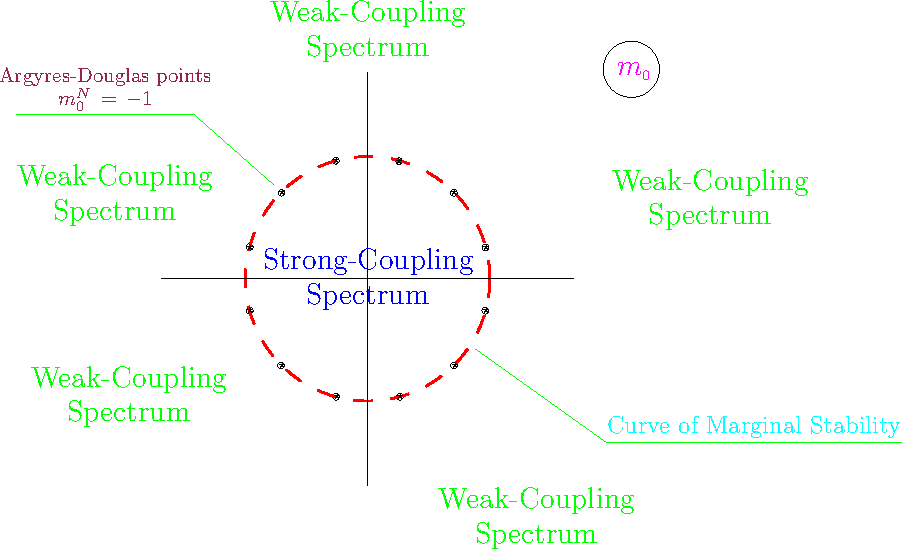
\includegraphics[width=10.0cm]{mplane.pdf}
\end{center}

\end{slide}


%%%%%%%%%%%%%%%%%%%%%%%%%%%%%%%%%%%%%%%%%%%%%%%%%%%%%%%%%%%%%%%%%%%%%%%%%%%%%%%%%%%%%
%%%%%%%%%%%%%%%%%%%%%%%%%%%%%%%%%%%%%%%%%%%%%%%%%%%%%%%%%%%%%%%%%%%%%%%%%%%%%%%%%%%%%
\begin{slide}

%\vspace*{3cm}
\centerline{\Huge \textcolor{red}{What happens in the circle?}}

\liststepwise{
%%\step{
%%%\vspace{-2cm}
%%\begin{center}
%%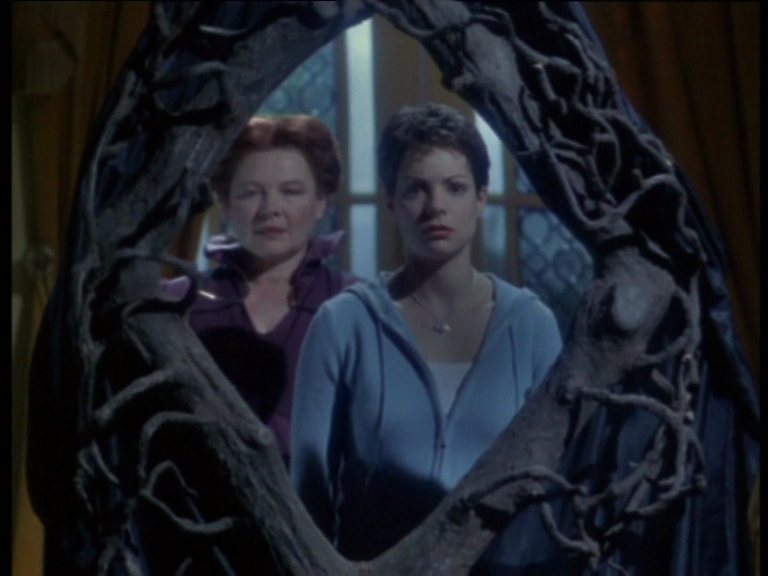
\includegraphics[width=10cm]{vlcsnap-2011-05-13-06h10m29s210.png}
%%\end{center}
%%}

\step{
%\vspace{-7cm}
\vspace{2cm}
\begin{center}
\Huge \textcolor{blue}{Mirror symmetry gives}

      \textcolor{blue}{the spectrum around the origin}
\end{center}
}
}

\end{slide}

%%%%%%%%%%%%%%%%%%%%%%%%%%%%%%%%%%%%%%%%%%%%%%%%%%%%%%%%%%%%%%%%%%%%%%%%%%%%%%%%%%%%%
%%%%%%%%%%%%%%%%%%%%%%%%%%%%%%%%%%%%%%%%%%%%%%%%%%%%%%%%%%%%%%%%%%%%%%%%%%%%%%%%%%%%%
\begin{slide}

\vspace*{-1cm}
\begin{center}
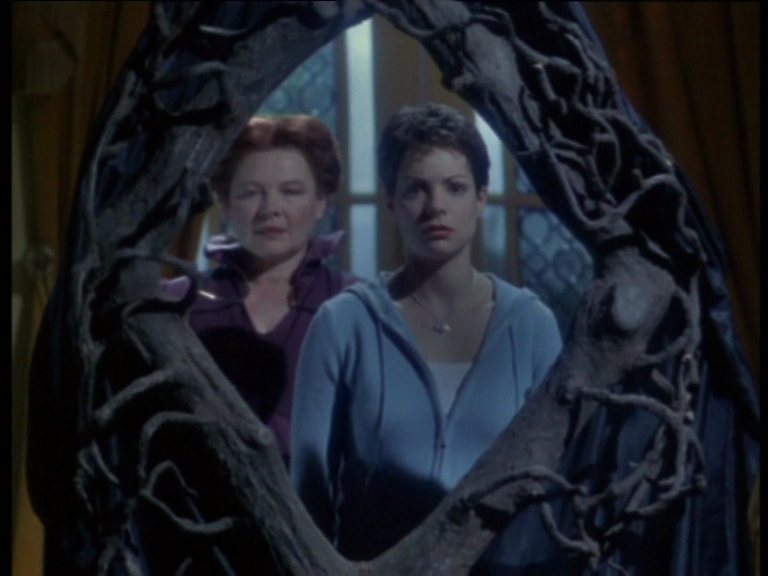
\includegraphics[width=12.8cm]{vlcsnap-2011-05-13-06h10m29s210.png}
\end{center}

\end{slide}


%%%%%%%%%%%%%%%%%%%%%%%%%%%%%%%%%%%%%%%%%%%%%%%%%%%%%%%%%%%%%%%%%%%%%%%%%%%%%%%%%%%%%
%%%%%%%%%%%%%%%%%%%%%%%%%%%%%%%%%%%%%%%%%%%%%%%%%%%%%%%%%%%%%%%%%%%%%%%%%%%%%%%%%%%%%
\begin{slide}

\centerline{\Huge Mirror Theory}
\vspace*{0.7cm}

[Vafa, Hori '00]
\[
	\W_\text{mirror}^\text{CP($N-1$)} ~~=~~
		-\, \frac{\Lambda}{2\pi}\, 
		\Bigl\{\, \sum_j X_j ~~+~~ \sum_j \frac{m_j}{\Lambda}\, \ln X_j \,\Bigr\}\,,
\]
subject to
\[
	\prod_j\, X_j ~~=~~ 1\,.
\]

\stepwise{
\step{
This theory at small $ m_0 $ predicts the existence of $ N $ kinks
\[
	\mbps ~~\approx~~ \Big|\, \frac{N}{2\pi} \lgr e^{2\pi i / N} \,-\, 1 \rgr \Lambda
			   ~~-~~ i\, m_j \,\Big|\,,
	\qquad\quad j~=~ 0,\,...,\, N-1\,\text.
\]
[Shifman, Yung '10]
}
}

\end{slide}


%%%%%%%%%%%%%%%%%%%%%%%%%%%%%%%%%%%%%%%%%%%%%%%%%%%%%%%%%%%%%%%%%%%%%%%%%%%%%%%%%%%%%
%%%%%%%%%%%%%%%%%%%%%%%%%%%%%%%%%%%%%%%%%%%%%%%%%%%%%%%%%%%%%%%%%%%%%%%%%%%%%%%%%%%%%
\begin{slide}

These are the states that become massless at the corresponding Argyres-Douglas points
$ \sigma_p ~=~ 	\sqrt[N] { 1 \,+\, m_0^N } \cdot e^{ 2\pi i p / N } ~=~ 0 $

\begin{center}
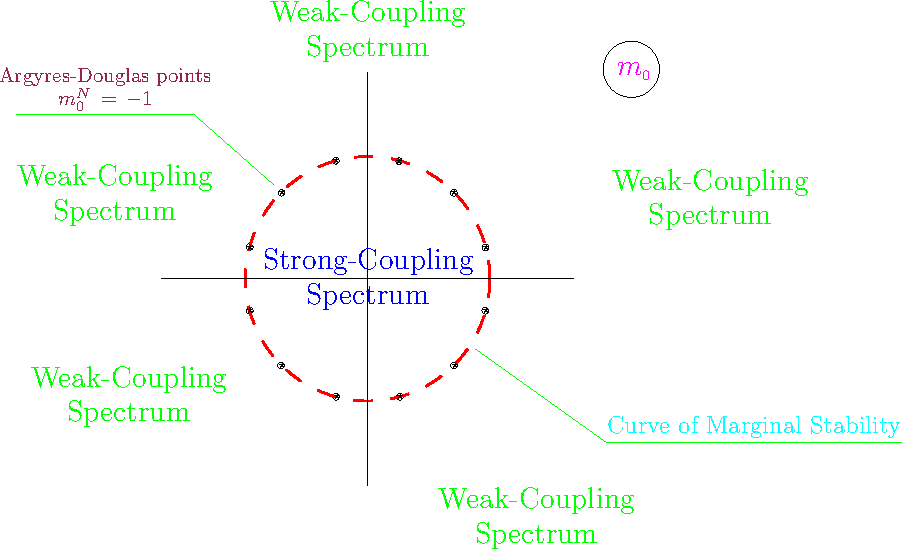
\includegraphics[width=10.0cm]{mplane.pdf}
\end{center}

Qualitatively this is seen from the formula
\[
	\mc{Z} ~~=~~  \text{``} \textcolor{blue}{
\W_\text{eff} ( \sigma_1 ) ~~-~~ \W_\text{eff} ( \sigma_0 )} \text{''} 
\]

\end{slide}


%%%%%%%%%%%%%%%%%%%%%%%%%%%%%%%%%%%%%%%%%%%%%%%%%%%%%%%%%%%%%%%%%%%%%%%%%%%%%%%%%%%%%
%%%%%%%%%%%%%%%%%%%%%%%%%%%%%%%%%%%%%%%%%%%%%%%%%%%%%%%%%%%%%%%%%%%%%%%%%%%%%%%%%%%%%
\begin{slide}

We prefer to work with our function $ U_0(m_0) $
{\tiny
\[
%
\label{unod}
	U_0 (m_0) ~~=~~ -\, \frac{1}{2\pi} \lgr e^{2\pi i / N} \,-\, 1 \rgr 
	\biggl\{\, N \sqrt[N] { 1 \,+\, m_0^N }  ~+~ 
	\sum_j\, m_j\, \ln  \lgr \sqrt[N] {1 \,+\,  m_0^N } \,-\, m_j \rgr  \biggr\}\,.
\]
}
\begin{center}
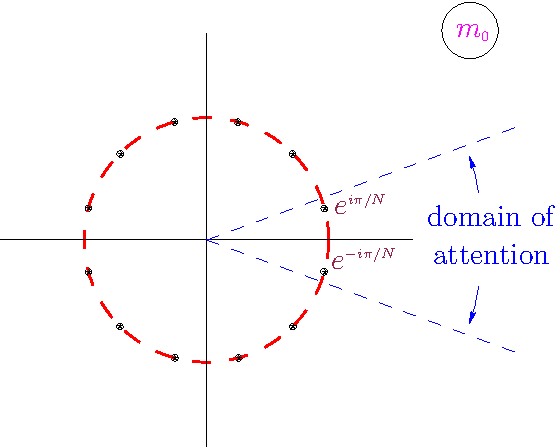
\includegraphics[width=8.0cm]{domain.pdf}
\end{center}
\[
\scriptstyle
	\mbps ~~=~~ U_0 (m_0) ~~+~~ i\, \vec{N} \cdot \vec{m}\,,
\]

\end{slide}


%%%%%%%%%%%%%%%%%%%%%%%%%%%%%%%%%%%%%%%%%%%%%%%%%%%%%%%%%%%%%%%%%%%%%%%%%%%%%%%%%%%%%
%%%%%%%%%%%%%%%%%%%%%%%%%%%%%%%%%%%%%%%%%%%%%%%%%%%%%%%%%%%%%%%%%%%%%%%%%%%%%%%%%%%%%
\begin{slide}

\centerline{\Large\textcolor{red}{General Criteria}}

\small
	We can now formulate the {\it requirements} for the spectrum of BPS states in the overall
	region of the complex mass parameter $ m_0 \,$:
\begin{itemize}
\item
	\emph{Quasi-classical limit} --- the spectrum at large $ m_0 $ and large excitation number $ n $
	must reproduce the semiclassical result:
\[
%\scriptstyle
\mbps ~~\simeq~~ \frac{N}{2\pi}\,
		( m_1 \,-\, m_0 ) \cdot \ln |m_0 |
	    ~~+~~
	i\, n \cdot ( m_1 \,-\, m_0 )\,;
\]

\item
	\emph{Argyres--Douglas point} --- the only states that survive when crossing from weak coupling 
	into the strong coupling region are those $ N $ states which become massless at the AD points;

\item
	\emph{Mirror spectrum} --- the latter $ N $ kinks must reflect the spectrum given by mirror 
	formula in the small $ m_0 $ limit:
\[
%\scriptstyle
	\mbps^{(j)} ~~\approx~~ \Big|\, -\, \frac{N}{2\pi} \lgr e^{2\pi i / N} \,-\, 1 \rgr 
			   ~~+~~ i\, m_j \,\Big|\,\text.
\]

\end{itemize}


\end{slide}


%%%%%%%%%%%%%%%%%%%%%%%%%%%%%%%%%%%%%%%%%%%%%%%%%%%%%%%%%%%%%%%%%%%%%%%%%%%%%%%%%%%%%
%%%%%%%%%%%%%%%%%%%%%%%%%%%%%%%%%%%%%%%%%%%%%%%%%%%%%%%%%%%%%%%%%%%%%%%%%%%%%%%%%%%%%
\begin{slide}

	Dorey's formula for the spectrum
\[
	\mc{Z} ~~=~~ \vec{T} \cdot \vec{m}{}_D ~~+~~ i\, \vec{N} \cdot \vec{m}
\]
	with $ \vec{N} ~=~ n\, \vec{T} $
	\emph{cannot} describe the set of the $ N $ states in the strong coupling region.

	The right answer is obtained by comparing our formula 
\[
\scriptstyle
	\mbps ~~=~~ U_0 (m_0) ~~+~~ i\, \vec{N} \cdot \vec{m}\,,
\]
\[
\scriptstyle
	U_0 (m_0) ~~=~~ -\, \frac{1}{2\pi} \lgr e^{2\pi i / N} \,-\, 1 \rgr 
	\biggl\{\, N \sqrt[N] { 1 \,+\, m_0^N }  ~+~ 
	\sum_j\, m_j\, \ln  \lgr \sqrt[N] {1 \,+\,  m_0^N } \,-\, m_j \rgr  \biggr\}\,
\]
	with the mirror result
\[
\scriptstyle
	\mbps^{(j)} ~~\approx~~ \Big|\, -\, \frac{N}{2\pi} \lgr e^{2\pi i / N} \,-\, 1 \rgr 
			   ~~+~~ i\, m_j \,\Big|\,
\]
	in the small mass limit. 

\end{slide}


%%%%%%%%%%%%%%%%%%%%%%%%%%%%%%%%%%%%%%%%%%%%%%%%%%%%%%%%%%%%%%%%%%%%%%%%%%%%%%%%%%%%%
%%%%%%%%%%%%%%%%%%%%%%%%%%%%%%%%%%%%%%%%%%%%%%%%%%%%%%%%%%%%%%%%%%%%%%%%%%%%%%%%%%%%%
\begin{slide}
	Near the origin we obtain
\[
	\mbps ~~\approx~~ -\, \frac{N}{2\pi} \lgr e^{2\pi i / N} \,-\, 1 \rgr ~~+~~ i\, \vec{N} \cdot \vec{m}\,,
\]
	The spectrum for the strong coupling area then is found to be
\[
\label{scpn}
	\vec{N} ~~=~~ 
			\quad
				\begin{array}{l} 
					(\, 1,~~~   0,~~~   0,~~~ ...,~~ 0 \,)\,, \\[1.5mm]
					(\, 0,~~~   1,~~~   0,~~~ ...,~~ 0 \,)\,, \\[1.5mm]
					(\, 0,~~~   0,~~~   1,~~~ ...,~~ 0 \,)\,, \\[0.5mm]
					\quad\quad.\quad.\quad.\quad.         \\
					(\, 0,~~~   0,~~~   0,~~~ ...,~~ 1 \,)\,.
				\end{array} 
\]
\vspace{-0.8cm}
\stepwise{
\step{\textcolor{red}{
	Precisely one of these states becomes massless at each corresponding AD point}.
}

\step{	Neither can this spectrum be described by the Dorey's formula, nor can it be fit
	into one tower of states
}
}

\end{slide}


%%%%%%%%%%%%%%%%%%%%%%%%%%%%%%%%%%%%%%%%%%%%%%%%%%%%%%%%%%%%%%%%%%%%%%%%%%%%%%%%%%%%%
%%%%%%%%%%%%%%%%%%%%%%%%%%%%%%%%%%%%%%%%%%%%%%%%%%%%%%%%%%%%%%%%%%%%%%%%%%%%%%%%%%%%%
\begin{slide}

	In order to describe the quasi-classical asymptotics
\[
%\scriptstyle
\mbps ~~\simeq~~ \frac{N}{2\pi}\,
		( m_1 \,-\, m_0 ) \cdot \ln |m_0 |
	    ~~+~~
	i\, n \cdot ( m_1 \,-\, m_0 )\,;
\]
	one has to introduce $ N - 1 $ towers
\begin{align*}
%
\notag
	\vec{N}_{(1)} & ~~=~~ (\, -\,n_{(1)} \,+\, 1,~~~~\; n_{(1)},~~~~\; 0,~~~~\; 0,~~~~\; ...,~~~~\; 0 \,)\,,  
	\\[2mm]
%
\notag
	\vec{N}_{(2)} & ~~=~~ (\, ~~~~~-\,n_{(2)},~~~~\; n_{(2)},~~~~\; 1,~~~~\; 0,~~~~\; ...,~~~~\; 0 \,)\,,
	\\[2mm]
%
	\vec{N}_{(3)} & ~~=~~ (\, ~~~~~-\,n_{(3)},~~~~\; n_{(3)},~~~~\; 0,~~~~\; 1,~~~~\; ...,~~~~\; 0 \,)\,,
	\\
%
\notag
	\qquad.\qquad.
	              & \qquad.\qquad.\qquad.\qquad.\qquad.\qquad.\qquad.
	\\
%
\notag
	\vec{N}_{(N-1)} & ~~=~~ (\, ~~-\,n_{(N-1)},~ n_{(N-1)},~~~~\, 0,~~~~\; 0,~~~~\; ...,~~~~\; 1 \,)\,.
\end{align*}

\stepwise{
\step{
\vspace{-0.2cm}
\centerline{\textcolor{magenta}{This is the spectrum which satisfies all three criteria}}
}
\step{
\vspace{-0.7cm}
\[
	\mbps ~~=~~ U_0 (m_0) ~~+~~ i\, n_{(k)} \cdot ( m_1 \,-\, m_0 ) ~~+~~ i\, m_k\,,
	\qquad {\scriptstyle k ~=~ 1,\,...,\, N-1\,}.
\]
}
}

\end{slide}


%%%%%%%%%%%%%%%%%%%%%%%%%%%%%%%%%%%%%%%%%%%%%%%%%%%%%%%%%%%%%%%%%%%%%%%%%%%%%%%%%%%%%
%%%%%%%%%%%%%%%%%%%%%%%%%%%%%%%%%%%%%%%%%%%%%%%%%%%%%%%%%%%%%%%%%%%%%%%%%%%%%%%%%%%%%
\begin{slide}

\vspace*{3.0cm} 
\begin{center}
\usefont{OT1}{lmvtt}{b}{n}\fontsize{35pt}{30pt}\selectfont
\bfseries
	Curves of Marginal Stability
\end{center}
\vspace*{2.0cm} 

\end{slide}


%%%%%%%%%%%%%%%%%%%%%%%%%%%%%%%%%%%%%%%%%%%%%%%%%%%%%%%%%%%%%%%%%%%%%%%%%%%%%%%%%%%%%
%%%%%%%%%%%%%%%%%%%%%%%%%%%%%%%%%%%%%%%%%%%%%%%%%%%%%%%%%%%%%%%%%%%%%%%%%%%%%%%%%%%%%
\begin{slide}
\vspace*{2cm}

	For each tower,
\[
	\mbps ~~=~~ U_0 (m_0) ~~+~~ i\, n_{(k)} \cdot ( m_1 \,-\, m_0 ) ~~+~~ i\, m_k\,,
	\qquad {\scriptstyle k ~=~ 1,\,...,\, N-1\,}.
\]
	there will be its own decay curve.
	The CMS condition is 
\[
	\text{Re}~~ \frac{ U_0 (m_0) ~~+~~ i\, m_k }
                         { m_1 ~~-~~ m_0 }    ~~=~~ 0\,. 
\]

	We will be drawing the curves in the $ m_0^N $ plane, otherwise a curve would
	repeat itself $ N $ times.

\end{slide}


%%%%%%%%%%%%%%%%%%%%%%%%%%%%%%%%%%%%%%%%%%%%%%%%%%%%%%%%%%%%%%%%%%%%%%%%%%%%%%%%%%%%%
%%%%%%%%%%%%%%%%%%%%%%%%%%%%%%%%%%%%%%%%%%%%%%%%%%%%%%%%%%%%%%%%%%%%%%%%%%%%%%%%%%%%%
\begin{slide}

	The first tower which we call \emph{primary} is special. 

\stepwise{
\step{
\textcolor{blue}{
	It represents the innermost curve of marginal stability. 
}
}

\step{
\textcolor{green}{
	It with necessity passes through the AD point, where it has a \textcolor{red}{cusp}.
}
}

\step{
\begin{center}
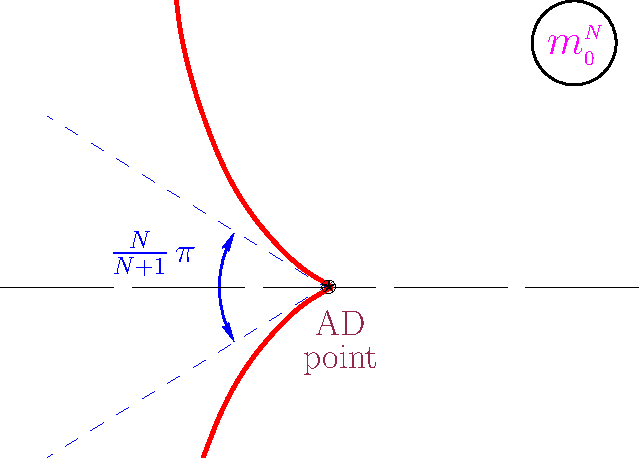
\includegraphics[width=6.0cm]{cusp.pdf}
\end{center}
}

\step{
\textcolor{magenta}{
	At infinite $ \origmath N $ the cusp flattens out, as the curves tend to circles.
}
}
}

\end{slide}


%%%%%%%%%%%%%%%%%%%%%%%%%%%%%%%%%%%%%%%%%%%%%%%%%%%%%%%%%%%%%%%%%%%%%%%%%%%%%%%%%%%%%
%%%%%%%%%%%%%%%%%%%%%%%%%%%%%%%%%%%%%%%%%%%%%%%%%%%%%%%%%%%%%%%%%%%%%%%%%%%%%%%%%%%%%
\begin{slide}

\centerline{\textcolor{red}{\Large The Curve for CP(1)}}

\vspace{-4.5cm}
\begin{center}
\hspace{2.5cm}
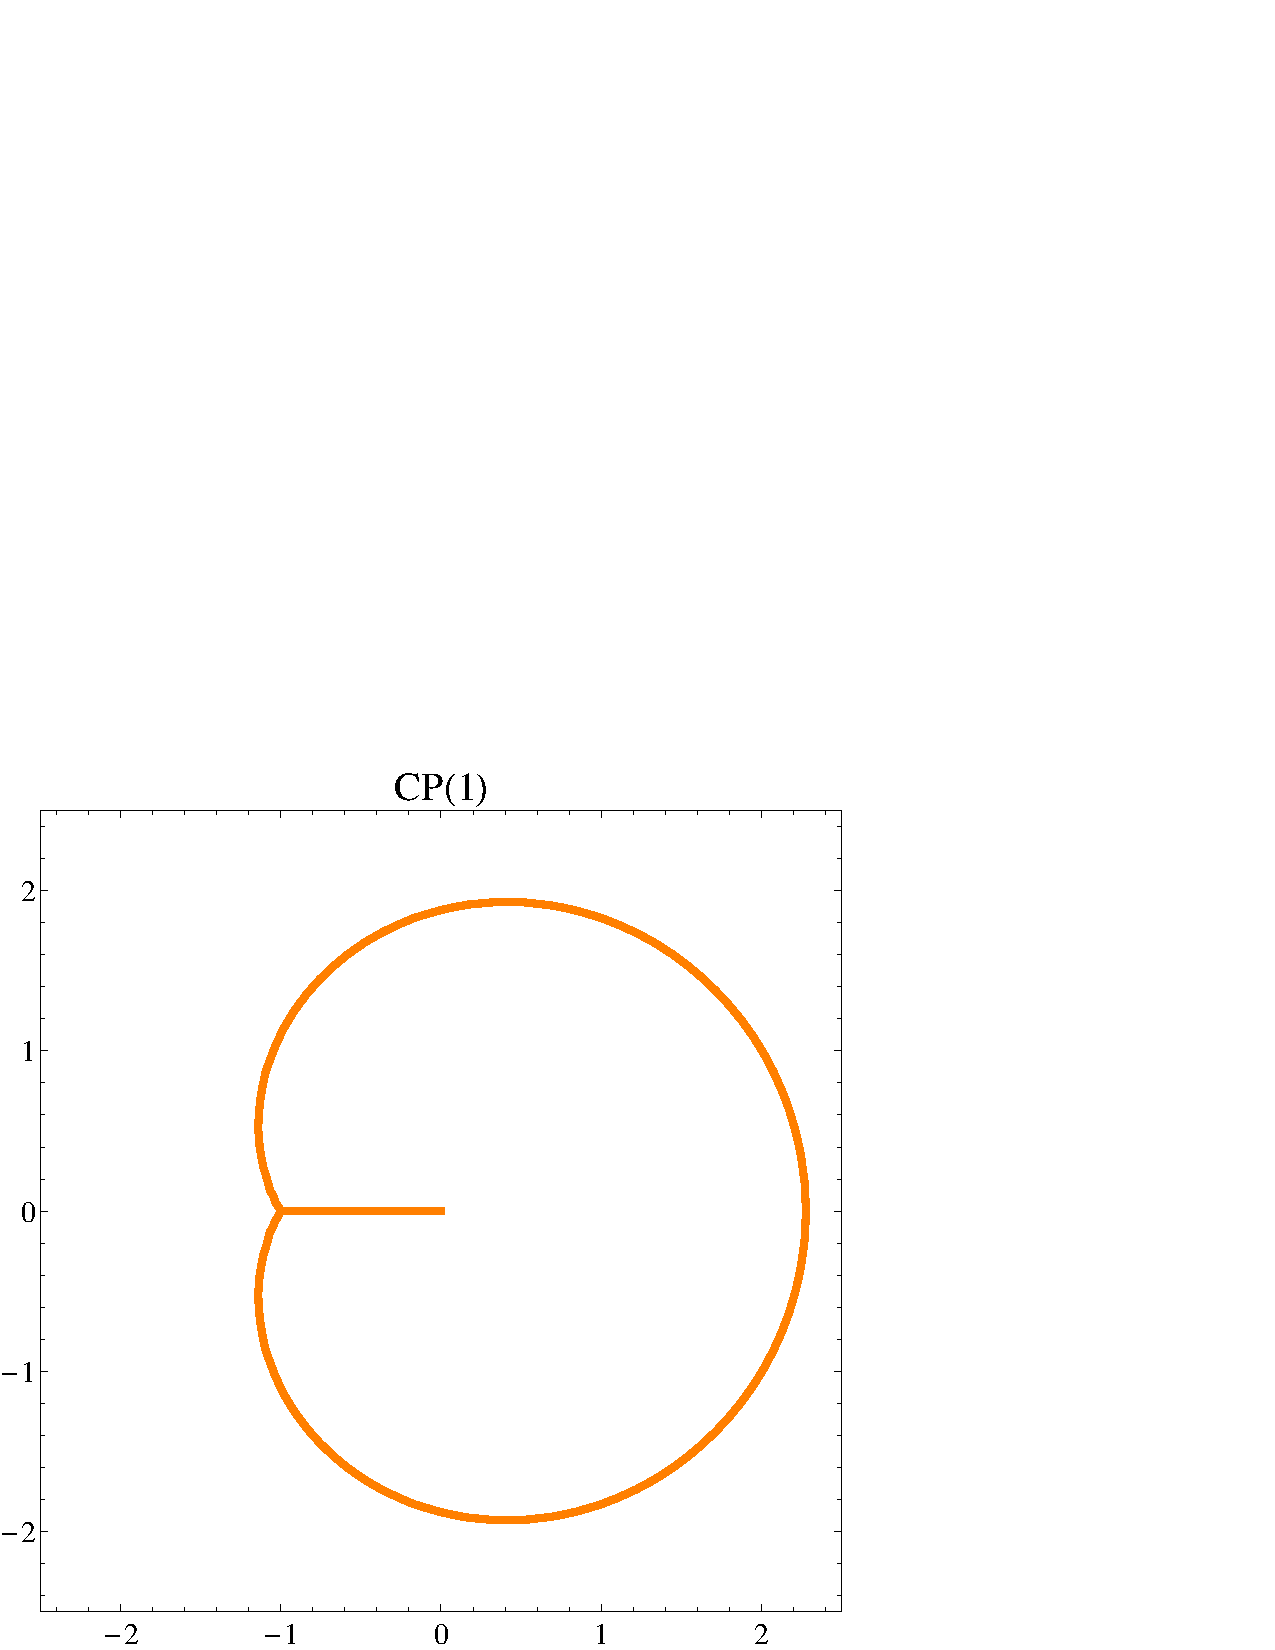
\includegraphics[width=9.0cm]{ccp1.pdf}
\end{center}

\end{slide}


%%%%%%%%%%%%%%%%%%%%%%%%%%%%%%%%%%%%%%%%%%%%%%%%%%%%%%%%%%%%%%%%%%%%%%%%%%%%%%%%%%%%%
%%%%%%%%%%%%%%%%%%%%%%%%%%%%%%%%%%%%%%%%%%%%%%%%%%%%%%%%%%%%%%%%%%%%%%%%%%%%%%%%%%%%%
\begin{slide}

\centerline{\textcolor{red}{\Large The Curves for CP(2)}}

\vspace{-4.5cm}
\begin{center}
\hspace{2.5cm}
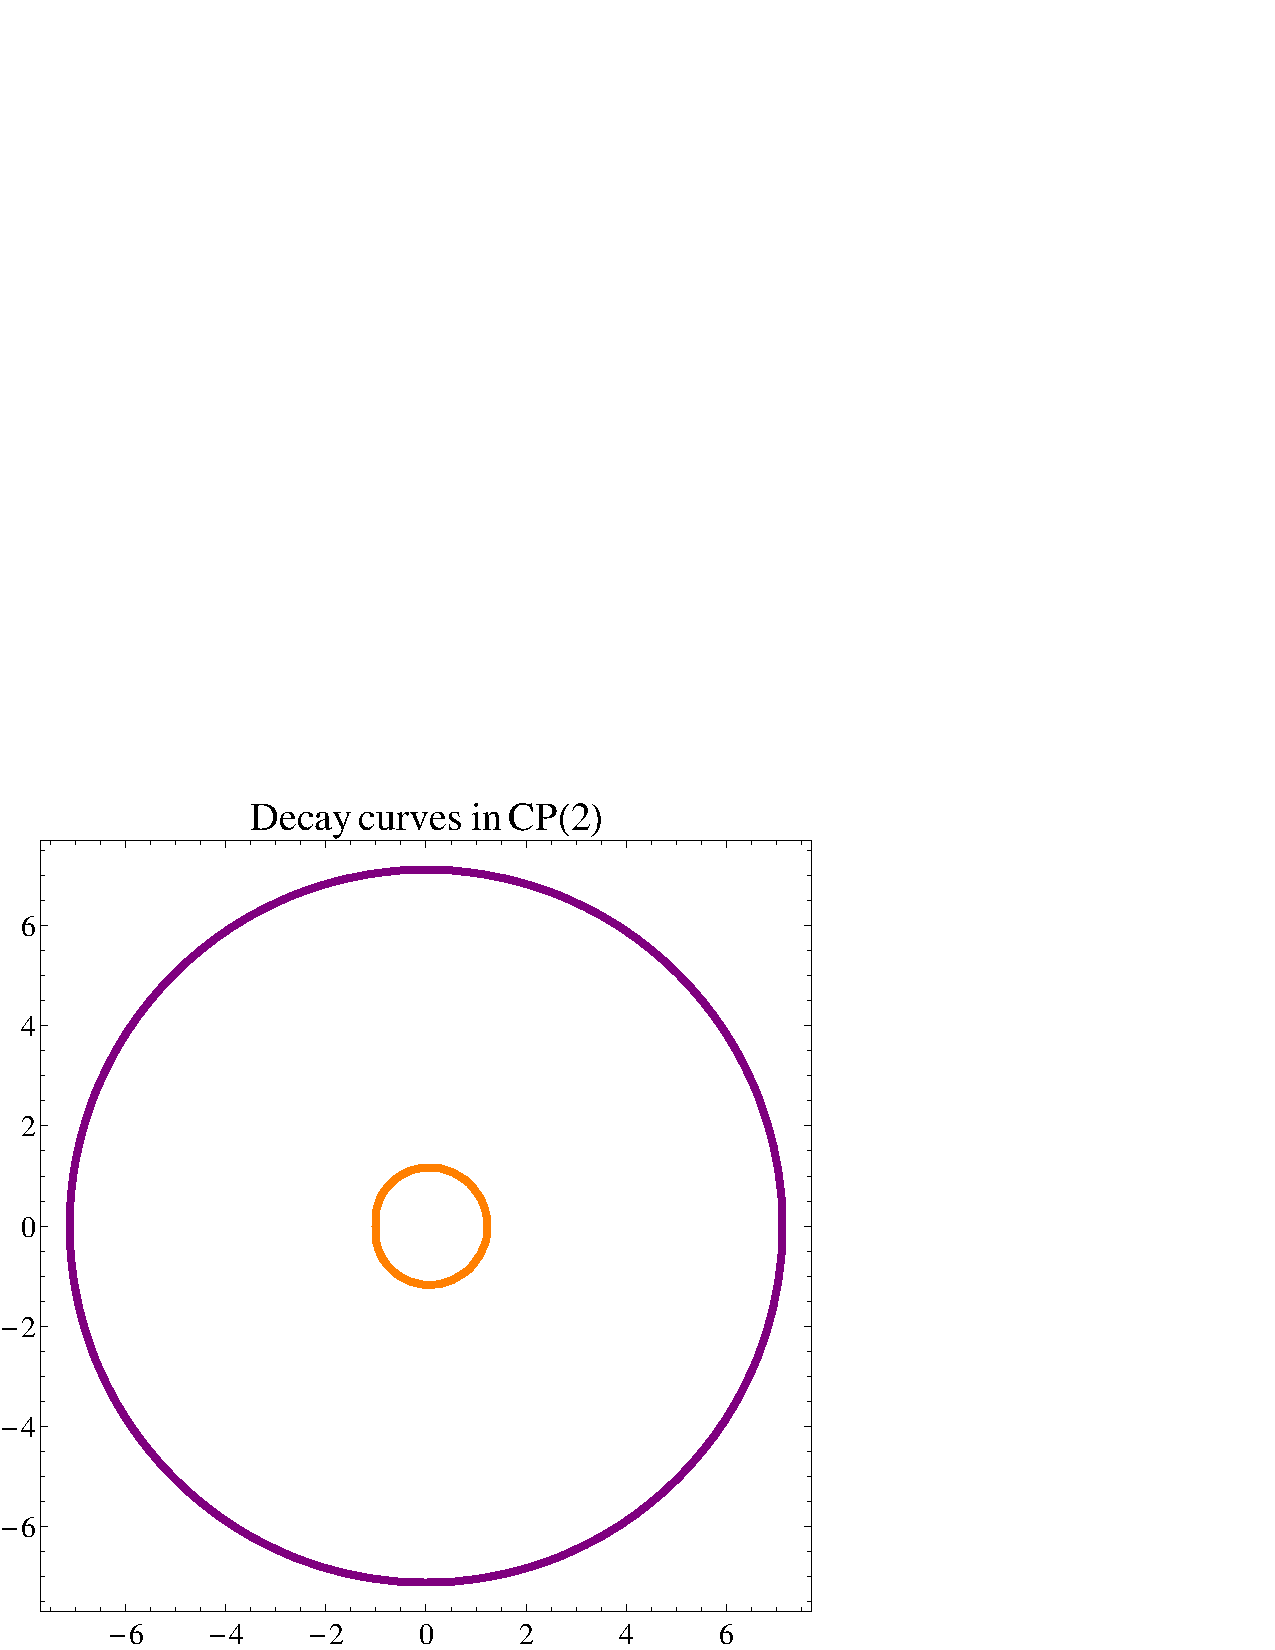
\includegraphics[width=9.0cm]{ccp2.pdf}
\end{center}

\centerline{\textcolor{green}{\small the plane has been rescaled in order to fit two curves}}

\end{slide}


%%%%%%%%%%%%%%%%%%%%%%%%%%%%%%%%%%%%%%%%%%%%%%%%%%%%%%%%%%%%%%%%%%%%%%%%%%%%%%%%%%%%%
%%%%%%%%%%%%%%%%%%%%%%%%%%%%%%%%%%%%%%%%%%%%%%%%%%%%%%%%%%%%%%%%%%%%%%%%%%%%%%%%%%%%%
\begin{slide}

\centerline{\textcolor{red}{\Large The Curves for CP(3)}}

\vspace{-4.5cm}
\begin{center}
\hspace{2.5cm}
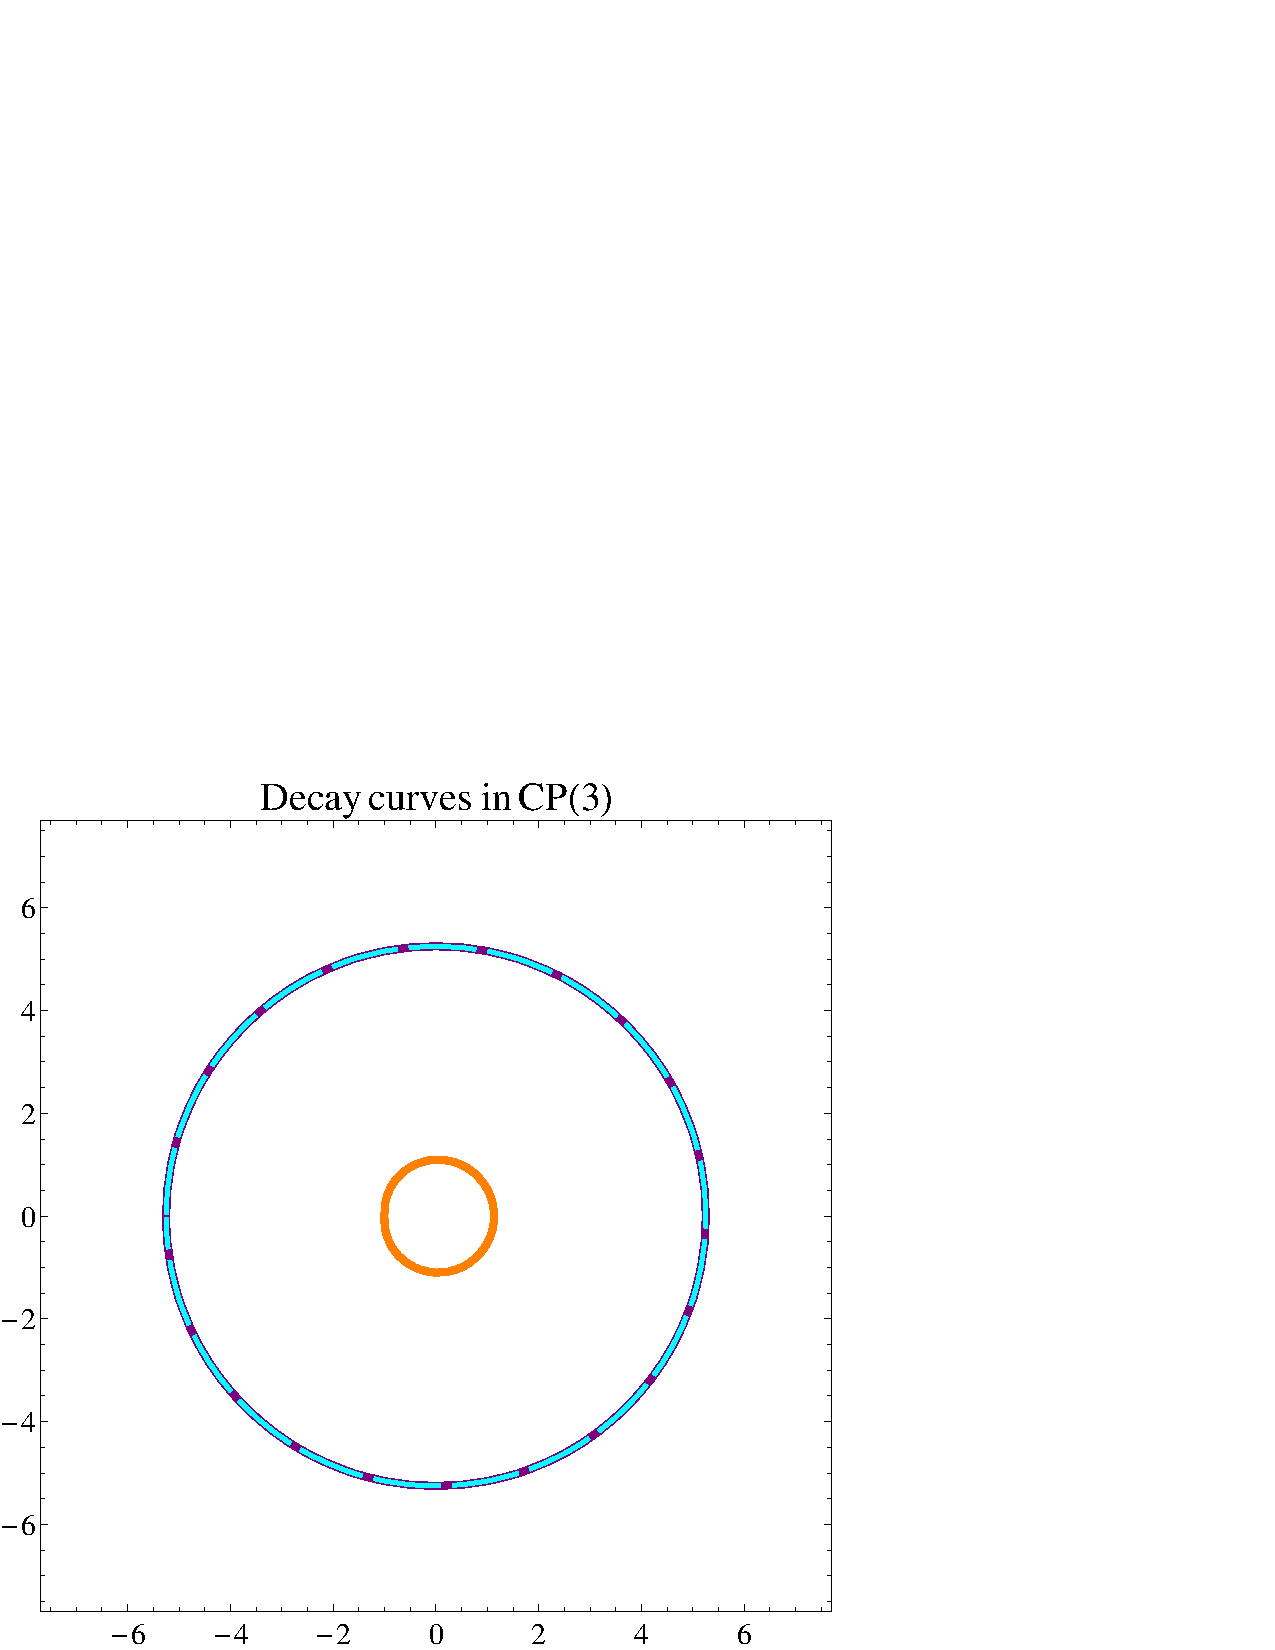
\includegraphics[width=9.0cm]{ccp3.pdf}
\end{center}

\centerline{\textcolor{green}{\small the plane has been rescaled in order to fit the curves}}

\end{slide}


%%%%%%%%%%%%%%%%%%%%%%%%%%%%%%%%%%%%%%%%%%%%%%%%%%%%%%%%%%%%%%%%%%%%%%%%%%%%%%%%%%%%%
%%%%%%%%%%%%%%%%%%%%%%%%%%%%%%%%%%%%%%%%%%%%%%%%%%%%%%%%%%%%%%%%%%%%%%%%%%%%%%%%%%%%%
\begin{slide}

\centerline{\textcolor{red}{\Large The Curves for CP(4)}}

\vspace{-4.5cm}
\begin{center}
\hspace{2.5cm}
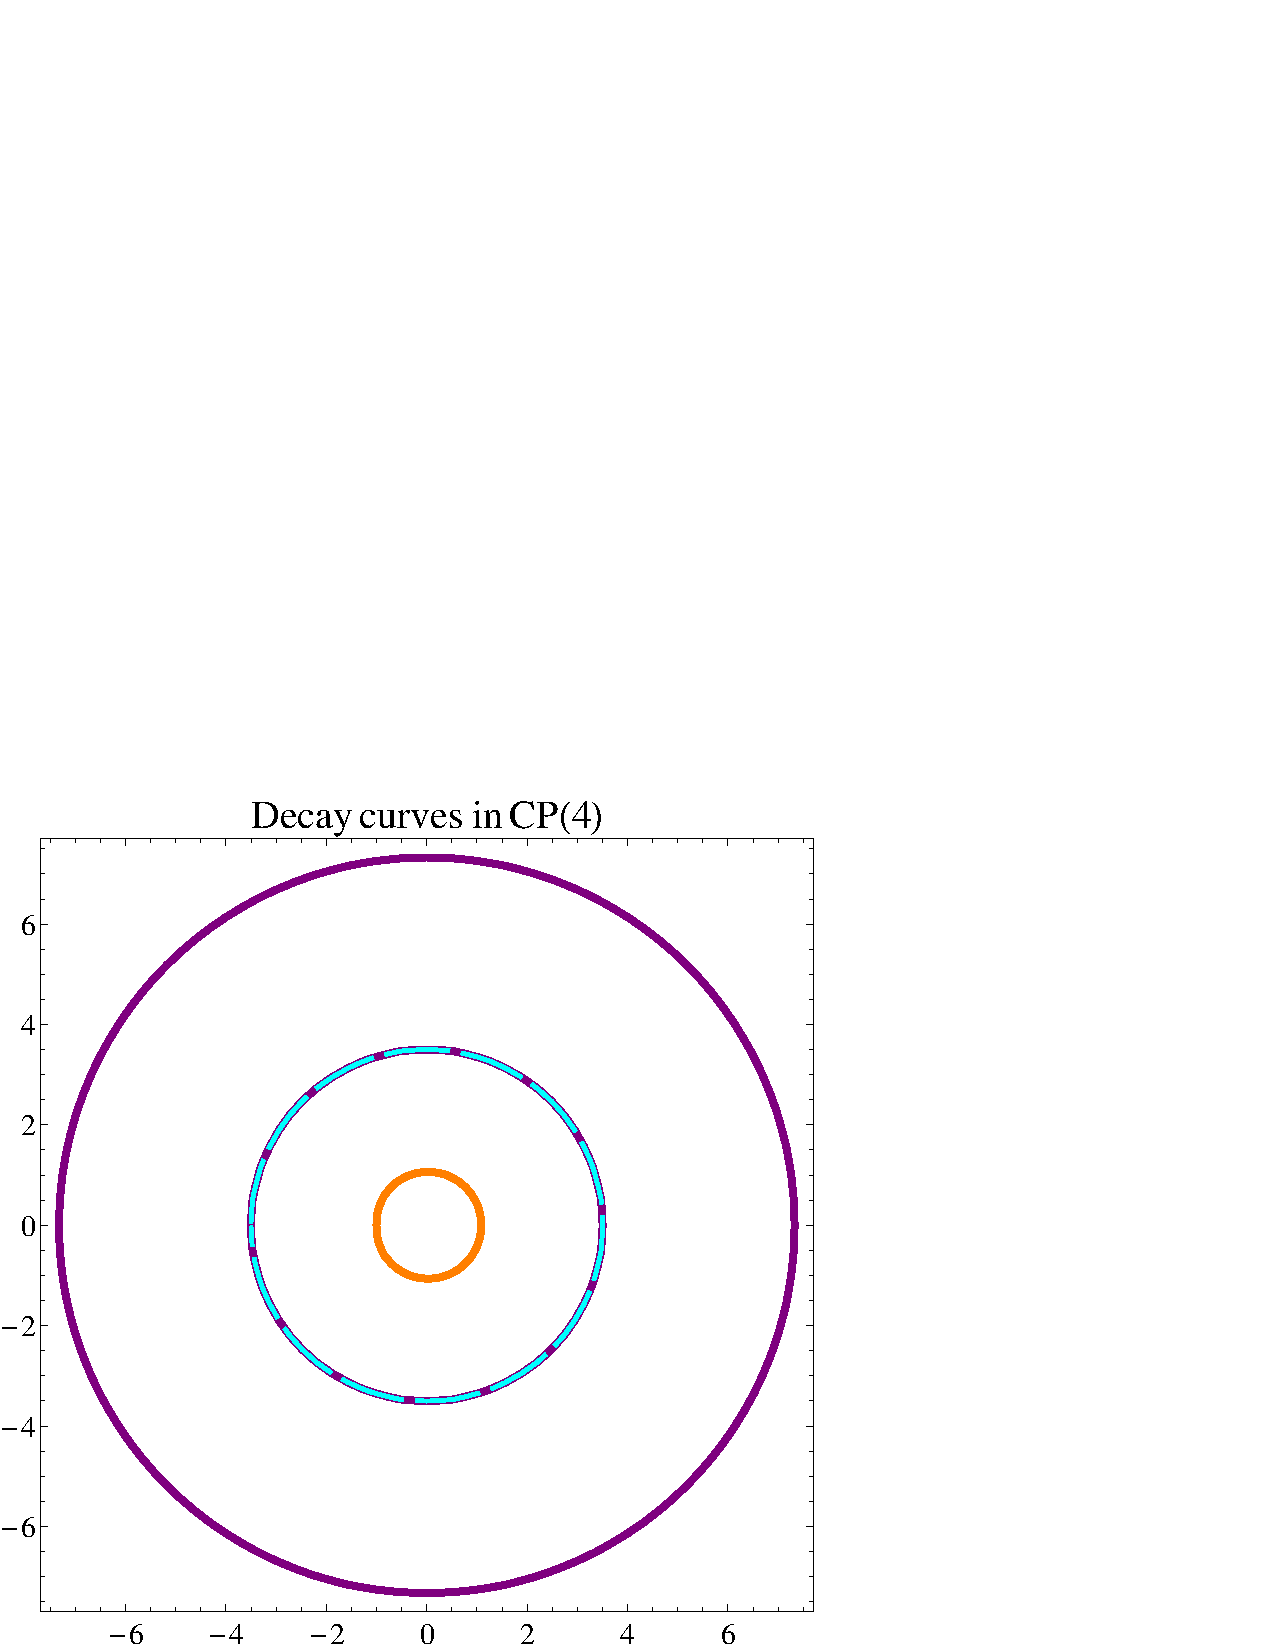
\includegraphics[width=9.0cm]{ccp4.pdf}
\end{center}

\centerline{\textcolor{green}{\small the plane has been rescaled in order to fit the curves}}

\end{slide}


%%%%%%%%%%%%%%%%%%%%%%%%%%%%%%%%%%%%%%%%%%%%%%%%%%%%%%%%%%%%%%%%%%%%%%%%%%%%%%%%%%%%%
%%%%%%%%%%%%%%%%%%%%%%%%%%%%%%%%%%%%%%%%%%%%%%%%%%%%%%%%%%%%%%%%%%%%%%%%%%%%%%%%%%%%%
\begin{slide}

\centerline{\textcolor{red}{\Large The Curves for CP(5)}}

\vspace{-4.5cm}
\begin{center}
\hspace{2.5cm}
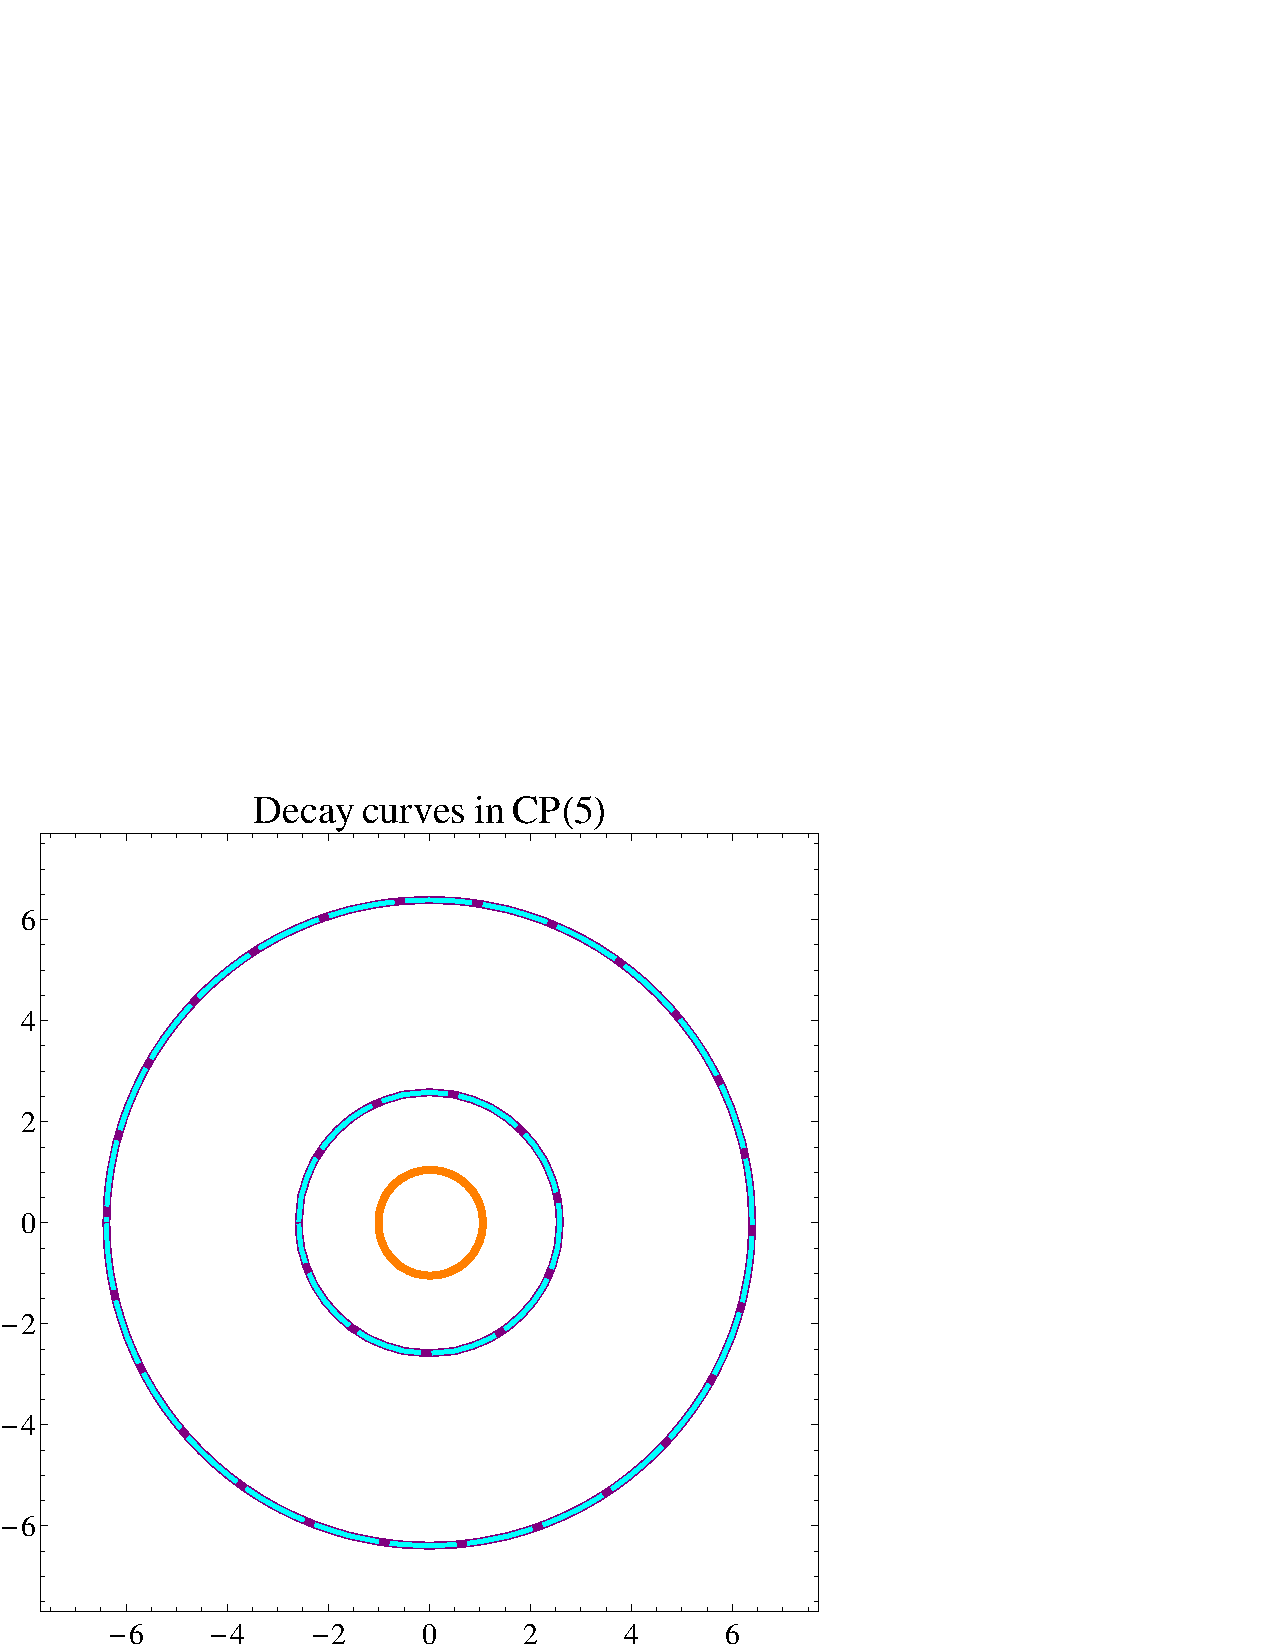
\includegraphics[width=9.0cm]{ccp5.pdf}
\end{center}

\centerline{\textcolor{green}{\small the plane has been rescaled in order to fit the curves}}

\end{slide}


%%%%%%%%%%%%%%%%%%%%%%%%%%%%%%%%%%%%%%%%%%%%%%%%%%%%%%%%%%%%%%%%%%%%%%%%%%%%%%%%%%%%%
%%%%%%%%%%%%%%%%%%%%%%%%%%%%%%%%%%%%%%%%%%%%%%%%%%%%%%%%%%%%%%%%%%%%%%%%%%%%%%%%%%%%%
\begin{slide}

\centerline{\textcolor{red}{\Large The Curves for CP(6)}}

\vspace{-4.5cm}
\begin{center}
\hspace{2.5cm}
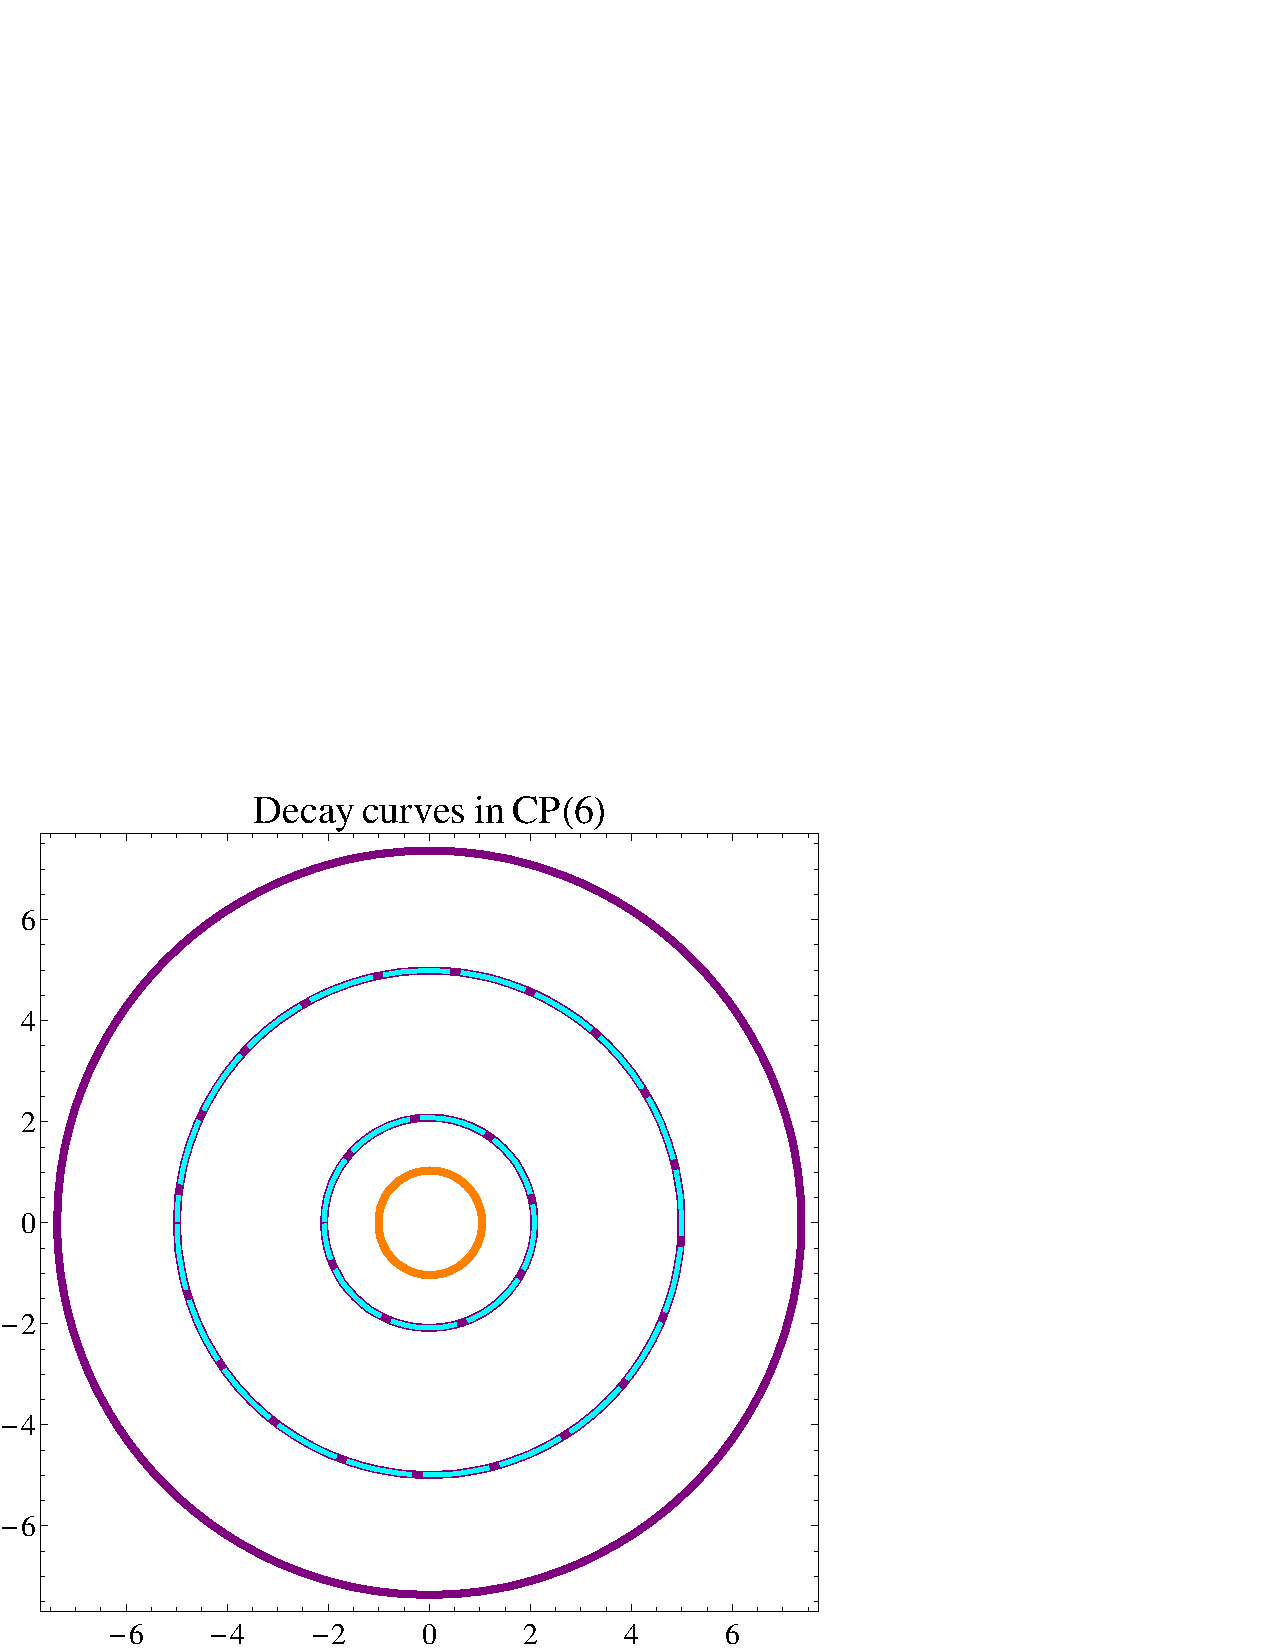
\includegraphics[width=9.0cm]{ccp6.pdf}
\end{center}

\centerline{\textcolor{green}{\small the plane has been rescaled in order to fit the curves}}

\end{slide}


%%%%%%%%%%%%%%%%%%%%%%%%%%%%%%%%%%%%%%%%%%%%%%%%%%%%%%%%%%%%%%%%%%%%%%%%%%%%%%%%%%%%%
%%%%%%%%%%%%%%%%%%%%%%%%%%%%%%%%%%%%%%%%%%%%%%%%%%%%%%%%%%%%%%%%%%%%%%%%%%%%%%%%%%%%%
\begin{slide}

\centerline{\textcolor{red}{\Large The Curves for CP(9)}}

\vspace{-4.5cm}
\begin{center}
\hspace{2.5cm}
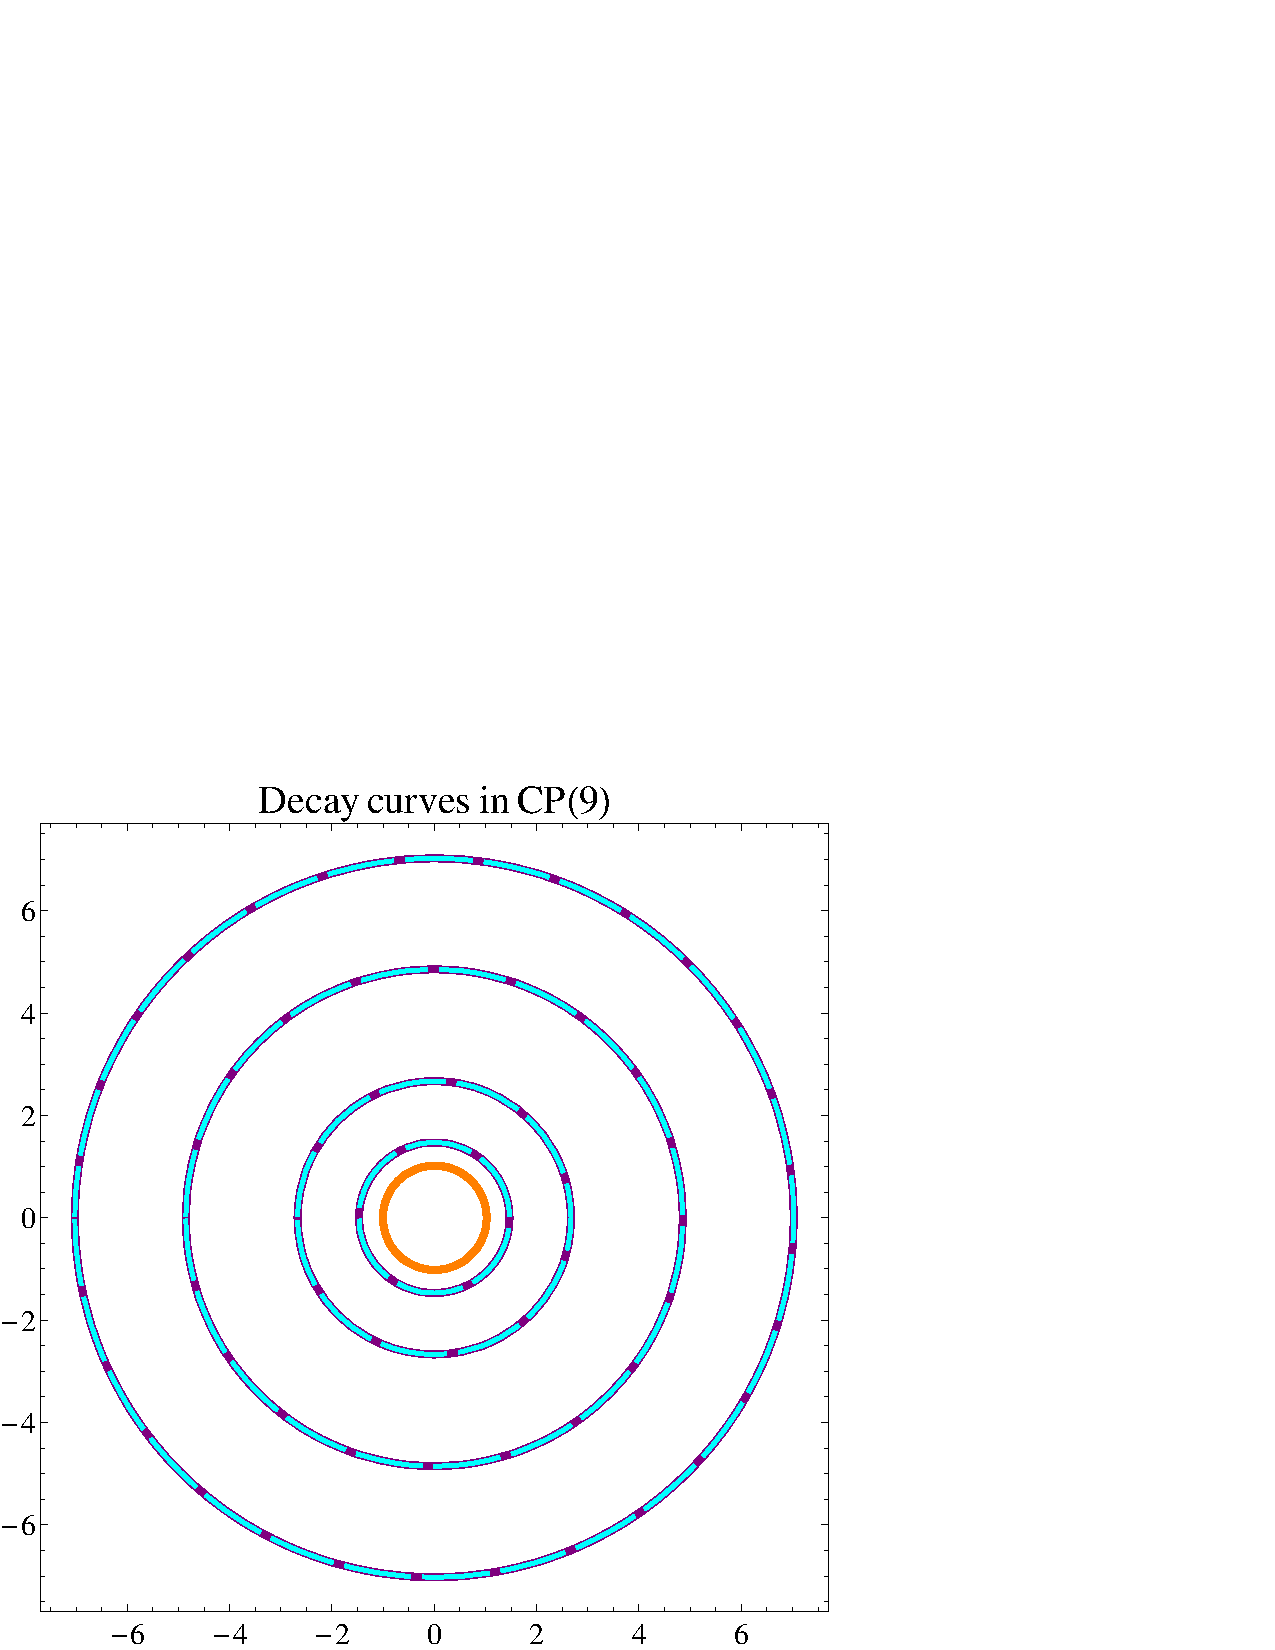
\includegraphics[width=9.0cm]{ccp9.pdf}
\end{center}

\centerline{\textcolor{green}{\small the plane has been rescaled in order to fit the curves}}

\end{slide}

%%%%%%%%%%%%%%%%%%%%%%%%%%%%%%%%%%%%%%%%%%%%%%%%%%%%%%%%%%%%%%%%%%%%%%%%%%%%%%%%%%%%%
%%%%%%%%%%%%%%%%%%%%%%%%%%%%%%%%%%%%%%%%%%%%%%%%%%%%%%%%%%%%%%%%%%%%%%%%%%%%%%%%%%%%%
\begin{slide}

\centerline{At larger $ N $ all the curves become circles with radii}
\vspace{-0.5cm}
\[
	\big| m_0 \big| ~~=~~ e^{ 1 \;-\; \cos\, \frac{\scriptstyle 2\, k \,-\, 1 } {\scriptstyle N }\, {\scriptstyle \pi} }\,,
	\qquad\qquad 
	\scriptstyle k ~=~ 1,\, ...,\, N\,-\,1\,\text.
\]

\stepwise{
\step{
\vspace{-5.5cm}
\begin{center}
\hspace{2.5cm}
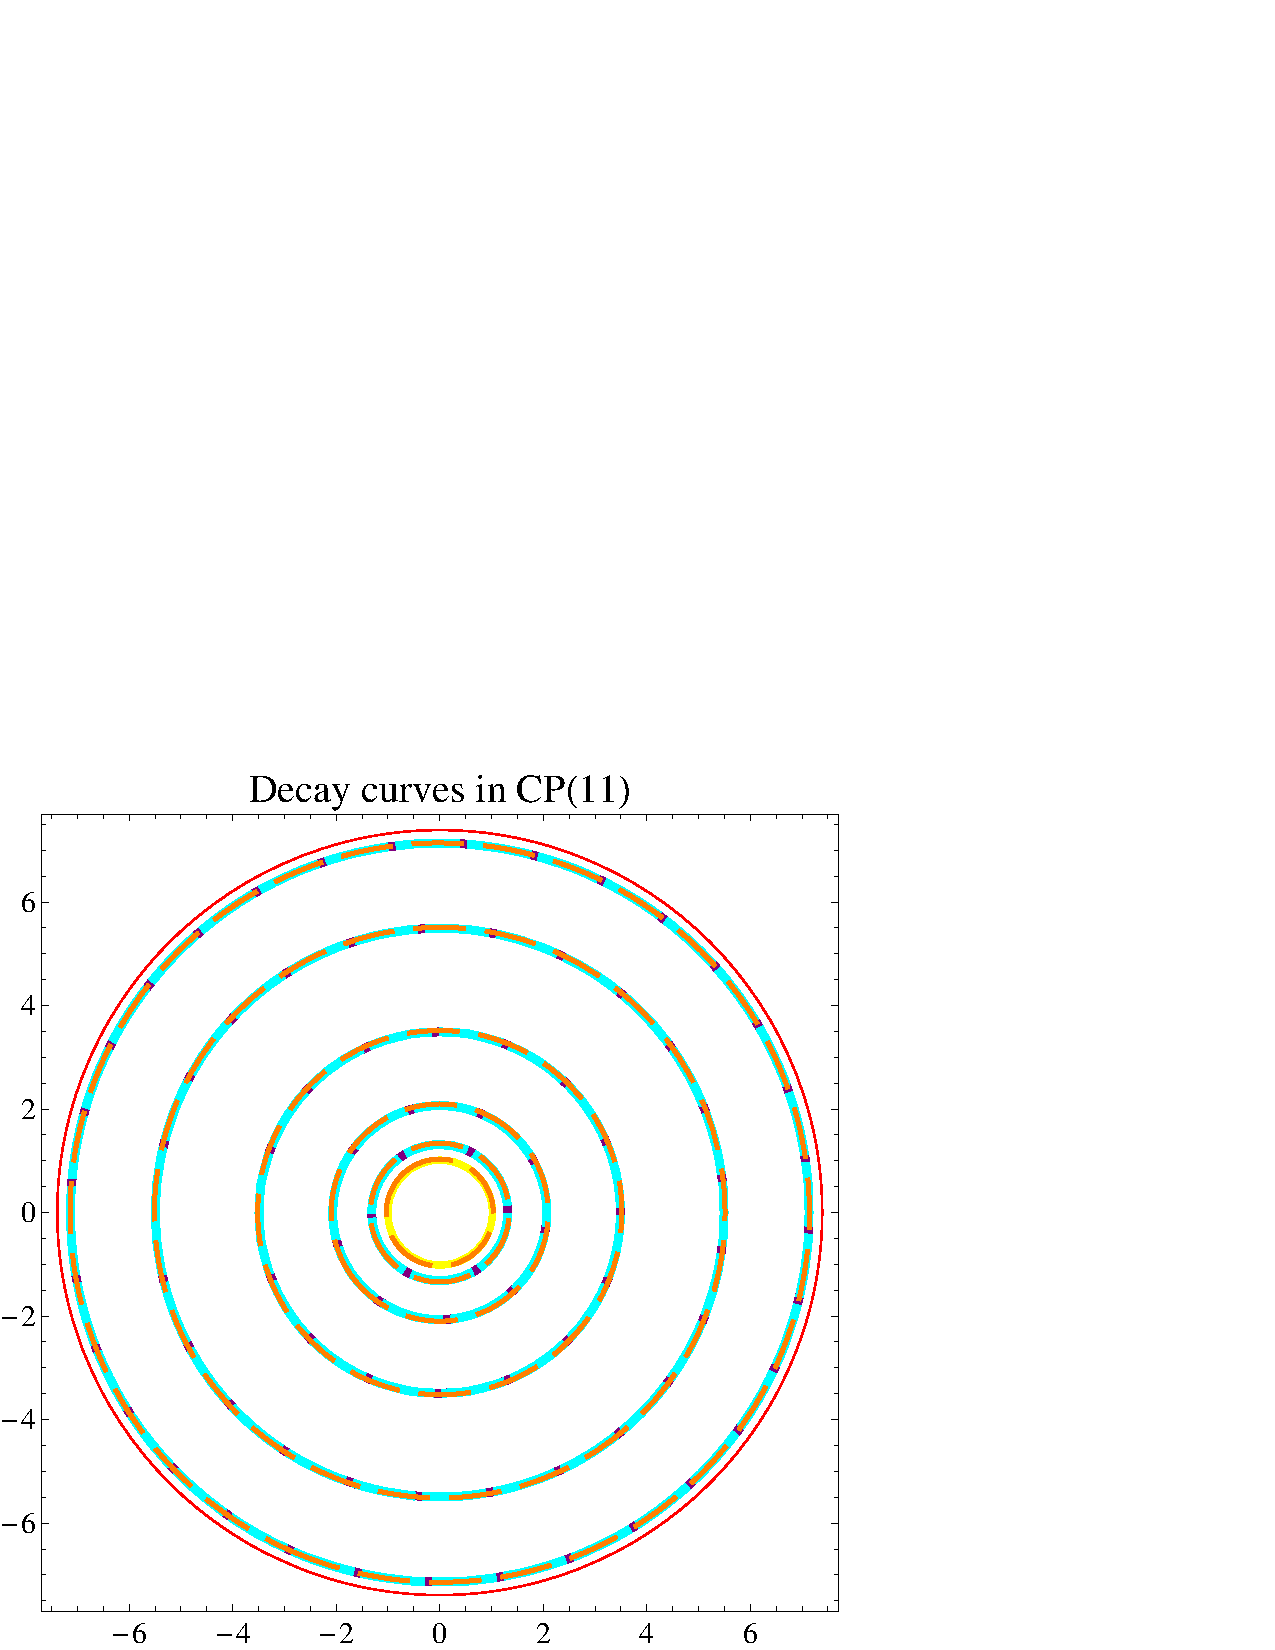
\includegraphics[width=9.0cm]{ccp11.pdf}
\end{center}

\centerline{\textcolor{green}{\small the plane has been rescaled in order to fit the curves}}
}
}

\end{slide}




%%%%%%%%%%%%%%%%%%%%%%%%%%%%%%%%%%%%%%%%%%%%%%%%%%%%%%%%%%%%%%%%%%%%%%%%%%%%%%%%%%%%%
%%%%%%%%%%%%%%%%%%%%%%%%%%%%%%%%%%%%%%%%%%%%%%%%%%%%%%%%%%%%%%%%%%%%%%%%%%%%%%%%%%%%%
\begin{slide}

\centerline{At larger $ N $ the curves fill the whole interval $ 1~~ ... ~~e^2 $}

\vspace{-4.5cm}
\begin{center}
\hspace{2.5cm}
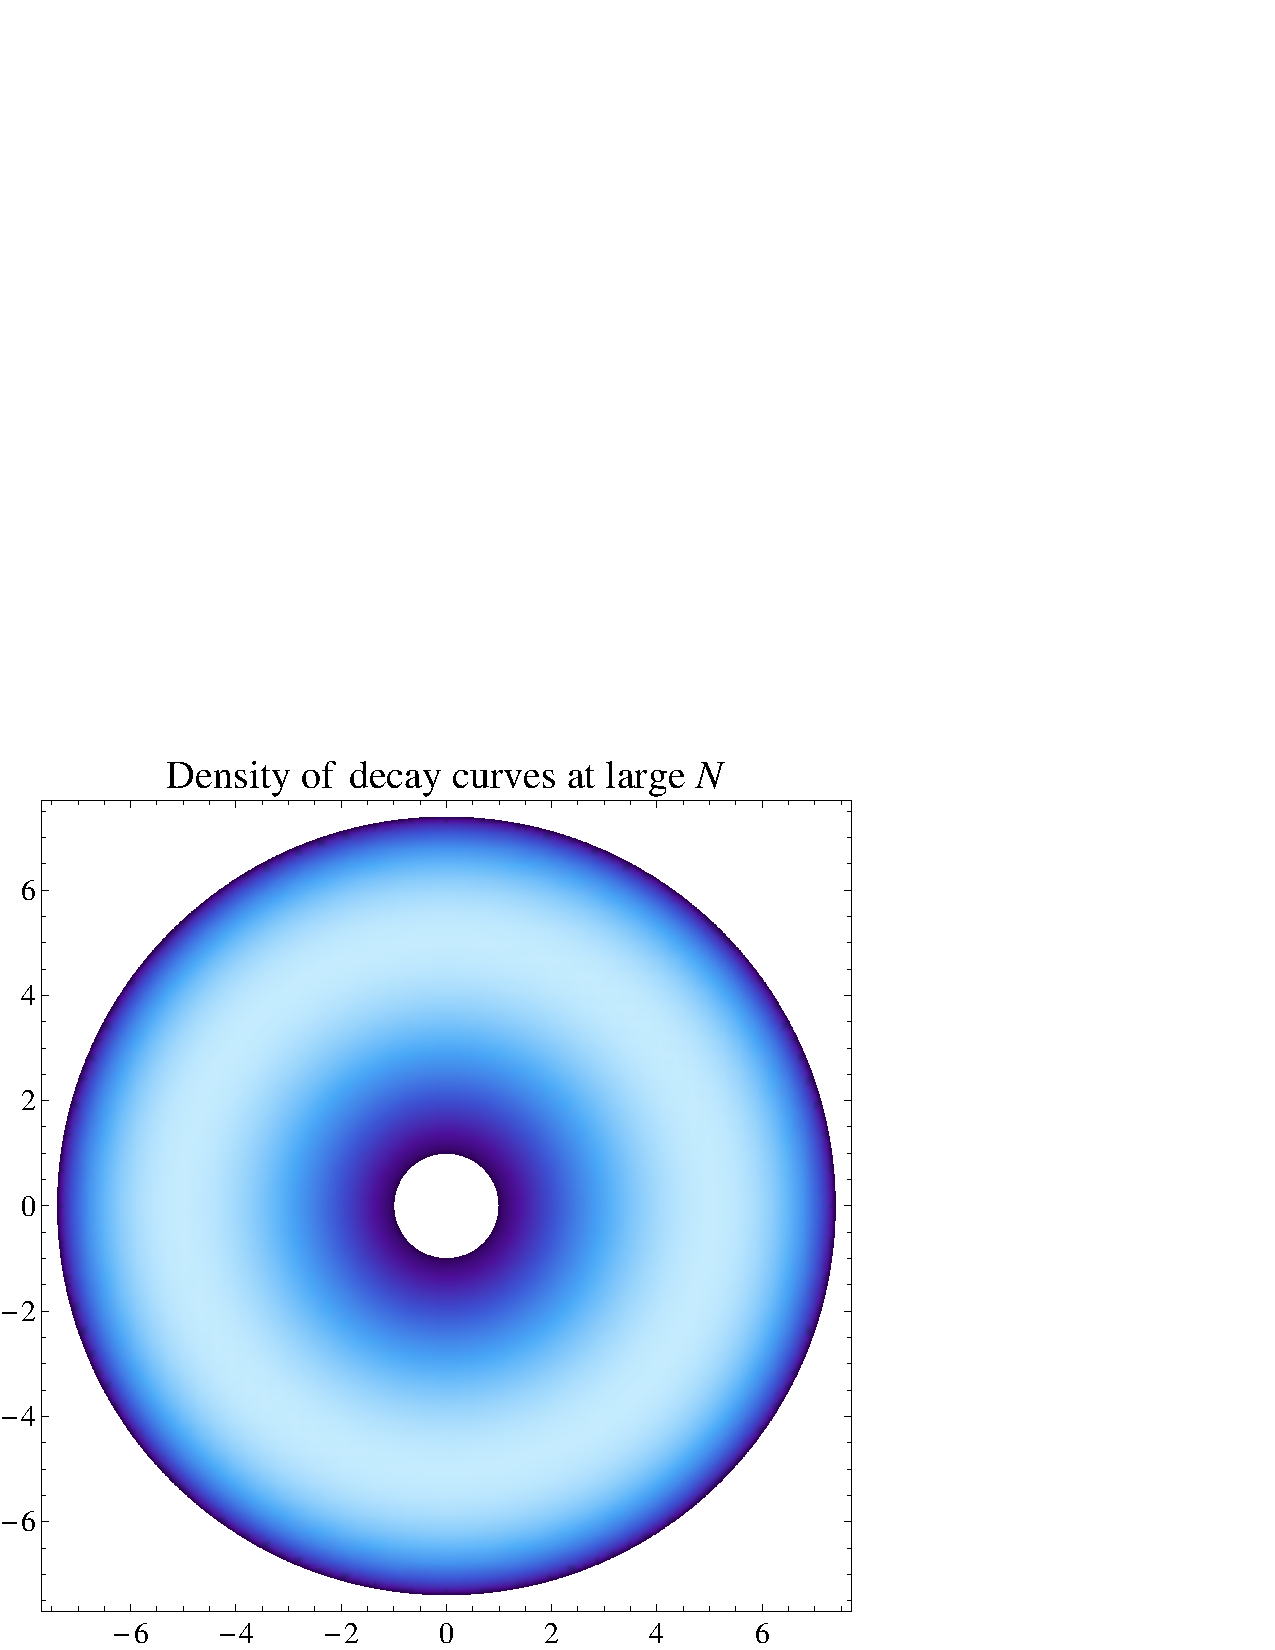
\includegraphics[width=9.0cm]{cmsdense.pdf}
\end{center}

\end{slide}


%%%%%%%%%%%%%%%%%%%%%%%%%%%%%%%%%%%%%%%%%%%%%%%%%%%%%%%%%%%%%%%%%%%%%%%%%%%%%%%%%%%%%
%%%%%%%%%%%%%%%%%%%%%%%%%%%%%%%%%%%%%%%%%%%%%%%%%%%%%%%%%%%%%%%%%%%%%%%%%%%%%%%%%%%%%
\begin{slide}

\centerline{\Large \textcolor{red}{Conclusion}}

\stepwise{
\step{
	Dorey's formula for the spectrum $ \mc{Z} ~=~ \vec{T} \cdot \vec{m}{}_D ~+~ i\, \vec{N} \cdot \vec{m} $
	is incomplete as it does not address the strong coupling region
	}

\step{\textcolor{red}{
	We formulated three criteria which must be met
}}

\step{
	\textcolor{magenta}{Based on the strong coupling spectrum, and AD points, we conclude that the weak-coupling spectrum
	must contain $ N - 1 $ towers}}\step{\textcolor{magenta}{:}
\small
\begin{align*}
%
\notag
	\vec{N}_{(1)} & ~~=~~ (\, -\,n_{(1)} \,+\, 1,~~~~\; n_{(1)},~~~~\; 0,~~~~\; 0,~~~~\; ...,~~~~\; 0 \,)\,,  
	\\[2mm]
%
\notag
	\vec{N}_{(2)} & ~~=~~ (\, ~~~~~-\,n_{(2)},~~~~\; n_{(2)},~~~~\; 1,~~~~\; 0,~~~~\; ...,~~~~\; 0 \,)\,,
	\\[2mm]
%
	\vec{N}_{(3)} & ~~=~~ (\, ~~~~~-\,n_{(3)},~~~~\; n_{(3)},~~~~\; 0,~~~~\; 1,~~~~\; ...,~~~~\; 0 \,)\,,
	\\
%
\notag
	\qquad.\qquad.
	              & \qquad.\qquad.\qquad.\qquad.\qquad.\qquad.\qquad.
	\\
%
\notag
	\vec{N}_{(N-1)} & ~~=~~ (\, ~~-\,n_{(N-1)},~ n_{(N-1)},~~~~\, 0,~~~~\; 0,~~~~\; ...,~~~~\; 1 \,)\,.
\end{align*}
}
}

\end{slide}


%%%%%%%%%%%%%%%%%%%%%%%%%%%%%%%%%%%%%%%%%%%%%%%%%%%%%%%%%%%%%%%%%%%%%%%%%%%%%%%%%%%%%
%%%%%%%%%%%%%%%%%%%%%%%%%%%%%%%%%%%%%%%%%%%%%%%%%%%%%%%%%%%%%%%%%%%%%%%%%%%%%%%%%%%%%
\begin{slide}

\begin{center}
	\textcolor{green}{In terms of masses}
\[
	\mbps ~~=~~ U_0 (m_0) ~~+~~ i\, n_{(k)} \cdot ( m_1 \,-\, m_0 ) ~~+~~ i\, m_k\,,
\]
	\textcolor{green}{for the towers {\small $  k ~=~ 1,~...,~ N - 1 $}}.
\end{center}

\stepwise{
\vspace{2cm}
\step{\centerline{\textcolor{red}{\Large Implications for SQCD are to be determined}}}
}

\end{slide}



%%%%%%%%%%%%%%%%%%%%%%%%%%%%%%%%%%%%%%%%%%%%%%%%%%%%%%%%%%%%%%%%%%%%%%%%%%%%%%%%%%%%%
%%%%%%%%%%%%%%%%%%%%%%%%%%%%%%%%%%%%%%%%%%%%%%%%%%%%%%%%%%%%%%%%%%%%%%%%%%%%%%%%%%%%%
\begin{slide}

\vspace*{-1cm}
\begin{center}
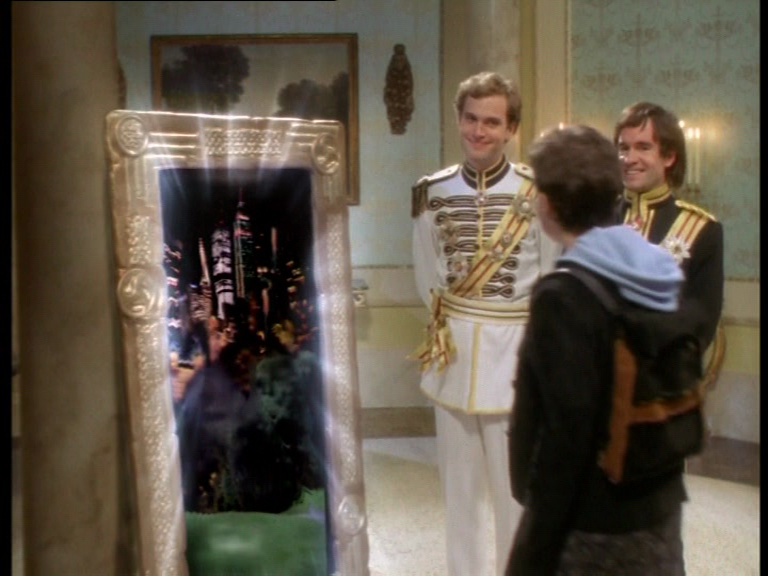
\includegraphics[width=12.8cm]{vlcsnap-2011-05-13-06h16m46s25.png}
\end{center}

\vspace{-6.5cm}
\stepwise{
\step{
\begin{center}
\usefont{OT1}{lmvtt}{b}{n}\fontsize{45pt}{30pt}\selectfont
\bfseries
\textcolor{yellow}{THANK YOU!}
\end{center}
}
}

\end{slide}

%%%%%%%%%%%%%%%%%%%%%%%%%%%%%%%%%%%%%%%%%%%%%%%%%%%%%%%%%%%%%%%%%%%%%%%%%%%%%%%%%%%%%
%%%%%%%%%%%%%%%%%%%%%%%%%%%%%%%%%%%%%%%%%%%%%%%%%%%%%%%%%%%%%%%%%%%%%%%%%%%%%%%%%%%%%
\begin{slide}

\end{slide}


%%%%%%%%%%%%%%%%%%%%%%%%%%%%%%%%%%%%%%%%%%%%%%%%%%%%%%%%%%%%%%%%%%%%%%%%%%%%%%%%%%%%%
%%%%%%%%%%%%%%%%%%%%%%%%%%%%%%%%%%%%%%%%%%%%%%%%%%%%%%%%%%%%%%%%%%%%%%%%%%%%%%%%%%%%%
\begin{slide}

\end{slide}


%%%%%%%%%%%%%%%%%%%%%%%%%%%%%%%%%%%%%%%%%%%%%%%%%%%%%%%%%%%%%%%%%%%%%%%%%%%%%%%%%%%%%
%%%%%%%%%%%%%%%%%%%%%%%%%%%%%%%%%%%%%%%%%%%%%%%%%%%%%%%%%%%%%%%%%%%%%%%%%%%%%%%%%%%%%
\begin{slide}

\end{slide}


%%%%%%%%%%%%%%%%%%%%%%%%%%%%%%%%%%%%%%%%%%%%%%%%%%%%%%%%%%%%%%%%%%%%%%%%%%%%%%%%%%%%%
%%%%%%%%%%%%%%%%%%%%%%%%%%%%%%%%%%%%%%%%%%%%%%%%%%%%%%%%%%%%%%%%%%%%%%%%%%%%%%%%%%%%%
\begin{slide}

\end{slide}


%%%%%%%%%%%%%%%%%%%%%%%%%%%%%%%%%%%%%%%%%%%%%%%%%%%%%%%%%%%%%%%%%%%%%%%%%%%%%%%%%%%%%
%%%%%%%%%%%%%%%%%%%%%%%%%%%%%%%%%%%%%%%%%%%%%%%%%%%%%%%%%%%%%%%%%%%%%%%%%%%%%%%%%%%%%
\begin{slide}

\end{slide}


%%%%%%%%%%%%%%%%%%%%%%%%%%%%%%%%%%%%%%%%%%%%%%%%%%%%%%%%%%%%%%%%%%%%%%%%%%%%%%%%%%%%%
%%%%%%%%%%%%%%%%%%%%%%%%%%%%%%%%%%%%%%%%%%%%%%%%%%%%%%%%%%%%%%%%%%%%%%%%%%%%%%%%%%%%%
\begin{slide}

\end{slide}


%%%%%%%%%%%%%%%%%%%%%%%%%%%%%%%%%%%%%%%%%%%%%%%%%%%%%%%%%%%%%%%%%%%%%%%%%%%%%%%%%%%%%
%%%%%%%%%%%%%%%%%%%%%%%%%%%%%%%%%%%%%%%%%%%%%%%%%%%%%%%%%%%%%%%%%%%%%%%%%%%%%%%%%%%%%
\begin{slide}

\end{slide}


%%%%%%%%%%%%%%%%%%%%%%%%%%%%%%%%%%%%%%%%%%%%%%%%%%%%%%%%%%%%%%%%%%%%%%%%%%%%%%%%%%%%%
%%%%%%%%%%%%%%%%%%%%%%%%%%%%%%%%%%%%%%%%%%%%%%%%%%%%%%%%%%%%%%%%%%%%%%%%%%%%%%%%%%%%%
\begin{slide}

\end{slide}


%%%%%%%%%%%%%%%%%%%%%%%%%%%%%%%%%%%%%%%%%%%%%%%%%%%%%%%%%%%%%%%%%%%%%%%%%%%%%%%%%%%%%
%%%%%%%%%%%%%%%%%%%%%%%%%%%%%%%%%%%%%%%%%%%%%%%%%%%%%%%%%%%%%%%%%%%%%%%%%%%%%%%%%%%%%
\begin{slide}

\end{slide}









\end{document}
\endinput

%%
%% End of file `talk.tex'.
